
\PassOptionsToPackage{hyphens,spaces,obeyspaces}{url}
\documentclass{iucrjournals}

\usepackage{amsmath}
\usepackage{amssymb}
\usepackage{graphicx}

% Multiplier-style "times" symbol for speedup factors etc.
% Uses a bold X so it does not visually collide with italic x in body text.
\newcommand{\xfac}{\mathbin{\boldsymbol{\times}}}

\DeclareUrlCommand\code{\urlstyle{tt}}
\emergencystretch=1em

% Number supplementary figures, tables and equations with an "S" prefix.
\renewcommand{\thefigure}{S\arabic{figure}}
\renewcommand{\thetable}{S\arabic{table}}
\renewcommand{\theequation}{S\arabic{equation}}

\title{Supplementary information for: TorchRef: An open-source PyTorch
  Framework for Crystallographic Refinement}

\author[a]{Hans-Peter Seidel%
  \IUCrCemaillink{hans.seidel@psi.ch}%
  \IUCrOrcidlink{0009-0005-4194-6833}}%
\author[a]{J\"org Standfuss%
  \IUCrCemaillink{joerg.standfuss@psi.ch}}%
\author[a]{Tobias Weinert%
  \IUCrCemaillink{tobias.weinert@psi.ch}}%

\affil[a]{Center for Life Sciences,
  Paul Scherrer Institut, 5232 Villigen PSI, Switzerland}

\begin{document}
\maketitle


%==============================================================================
\section*{Reading guide}
%==============================================================================

This supplement is in two parts. The first part presents the four
\textbf{Supplementary figures} referenced from the main manuscript: the
loss-weight calibration sweep (Fig.~S1), the
per-resolution TorchRef--reference R-factor comparison (Fig.~S2), the
cross-scorer validation (Fig.~S3), and the single-core wall-clock runtime
comparison (Fig.~S4). The second part,
\textbf{Supplementary methods}, is
an algorithmic reference for readers who wish to understand or extend
TorchRef's internals: parameterisations, structure factor calculation,
X-ray target functions, restraints, the AMBER target, the multi-dataset
infrastructure, loss aggregation, and the optimisation cycle.


%==============================================================================
\section*{Supplementary figures}
%==============================================================================

\begin{figure}[ht]
\begin{center}
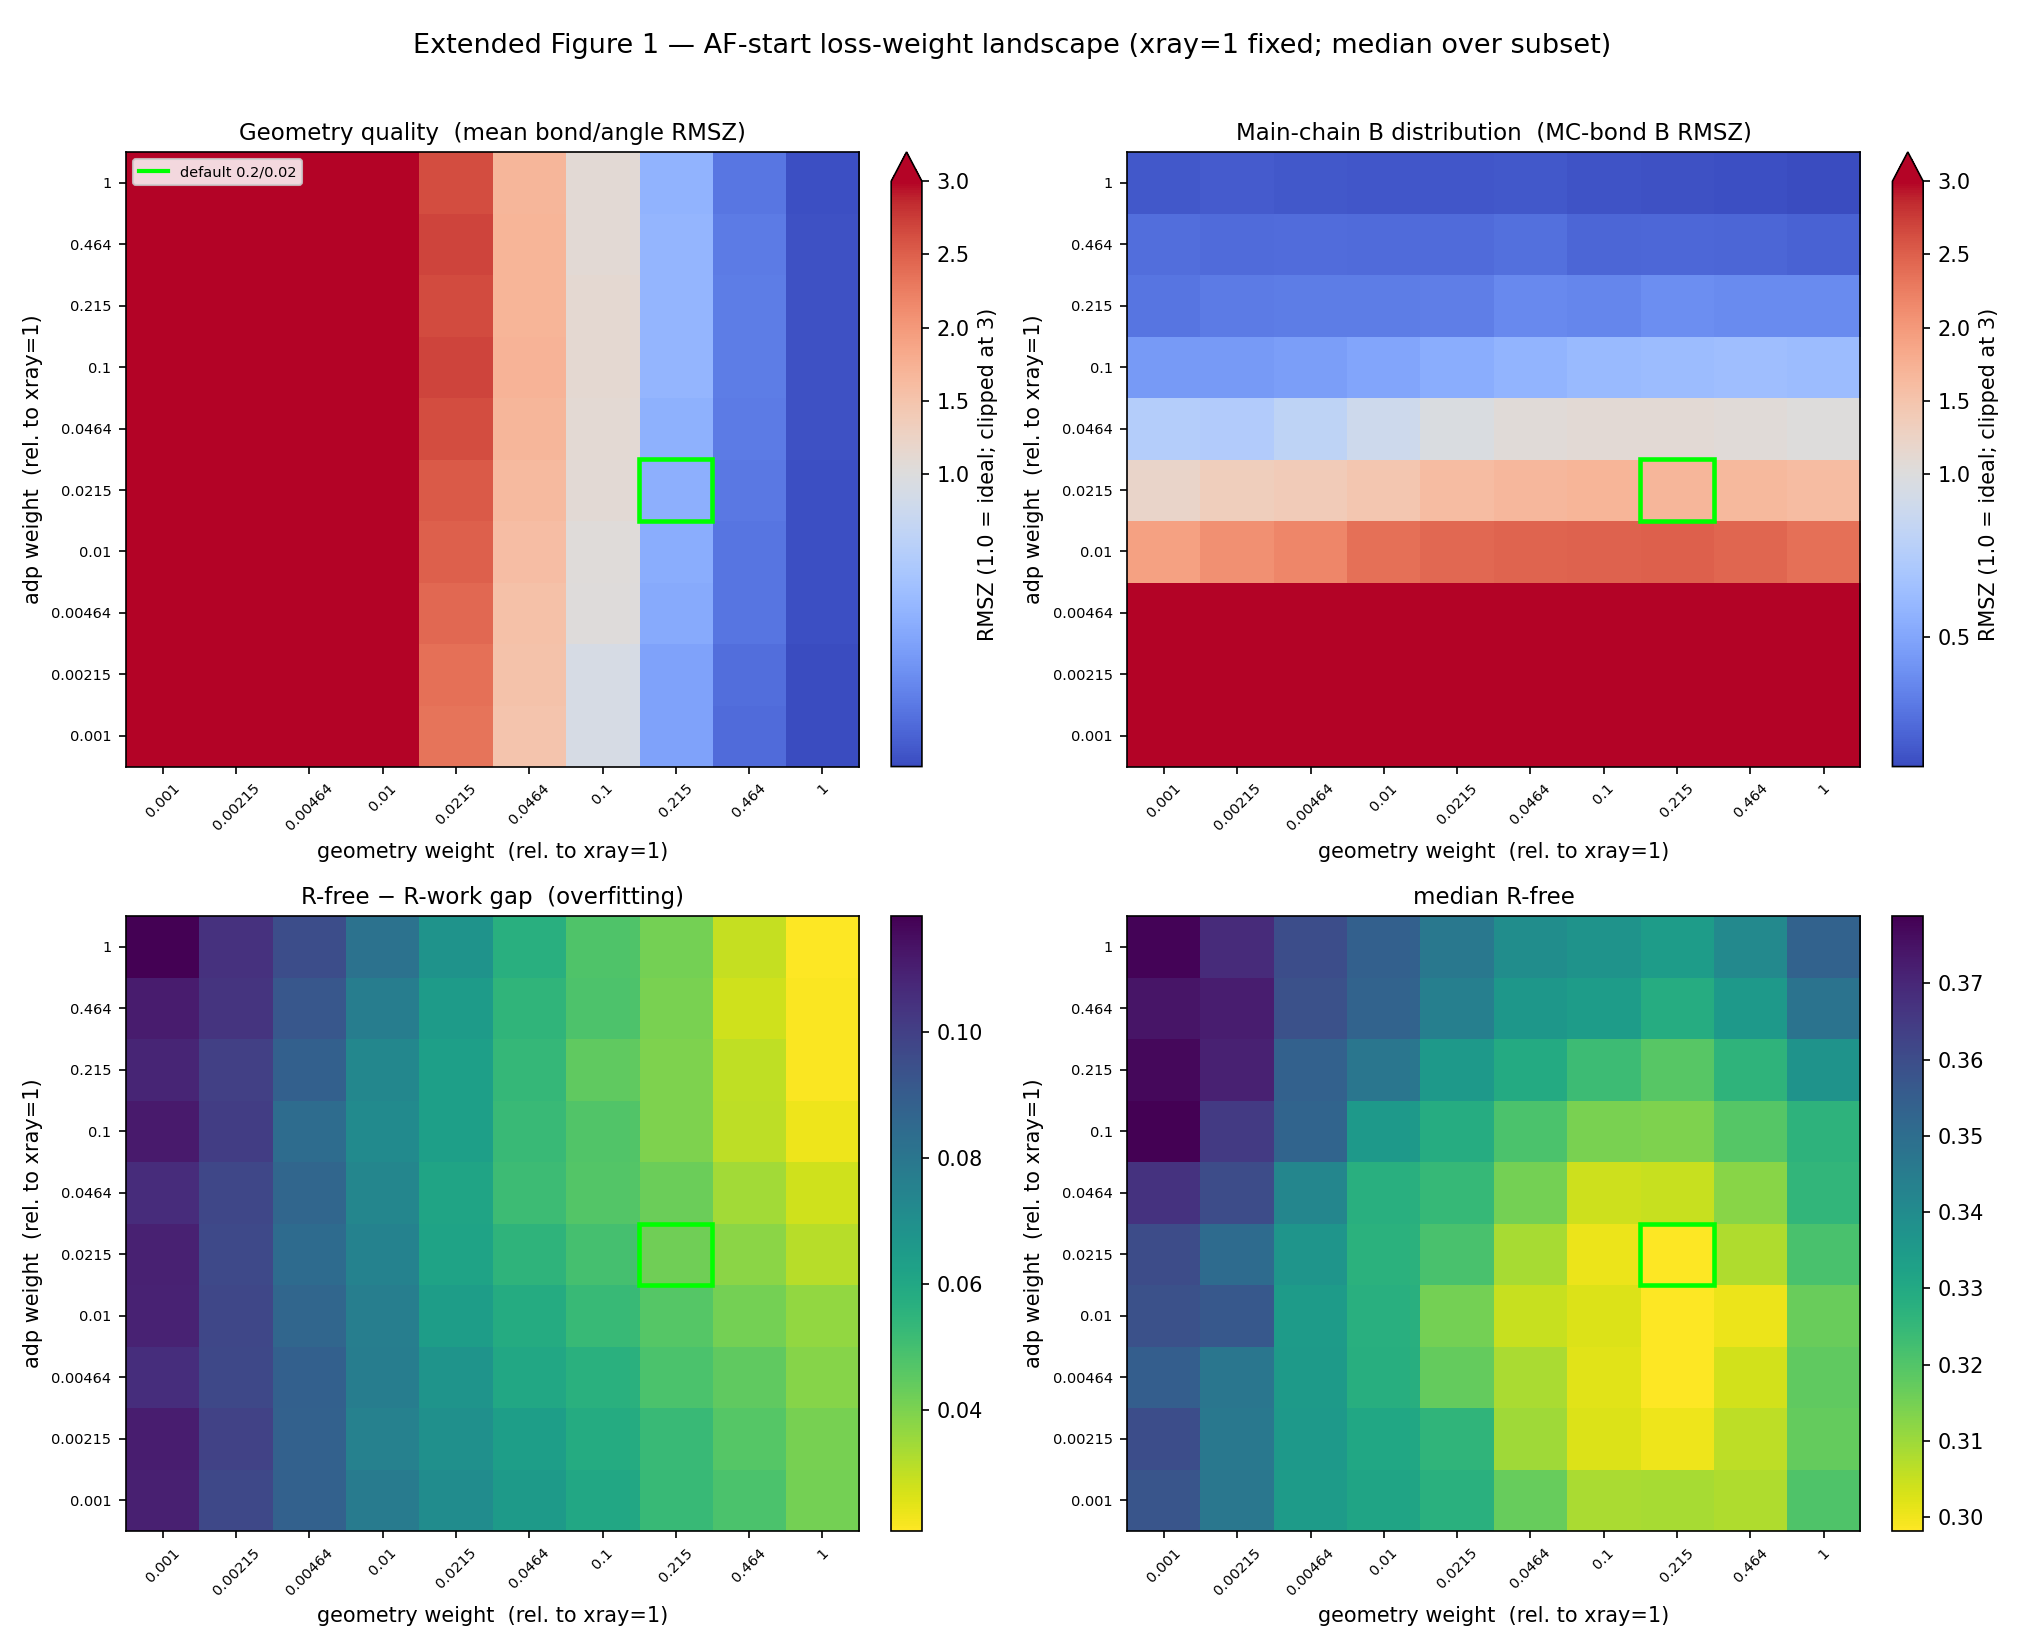
\includegraphics[width=\textwidth]{figS1.png}
\end{center}
\caption{%
  Loss-weight landscape on the AlphaFold benchmark, exploring the
  $(w_\mathrm{geometry},\,w_\mathrm{adp})$ plane at fixed
  $w_\mathrm{xray} = 1$.  Each heat-map cell is the median refinement
  outcome for a stratified subset of structures refined at that weight
  setting; the green box marks the TorchRef default
  $(w_\mathrm{geometry},\,w_\mathrm{adp}) = (0.2,\,0.02)$.
  Top-left: median bond/angle RMSZ (geometry quality).
  Top-right: main-chain bonded-B RMSZ (ADP distribution).
  Bottom-left: median $R_\mathrm{work}$--$R_\mathrm{free}$ gap (overfitting).
  Bottom-right: median $R_\mathrm{free}$.
  The default sits in a flat region of the
  ($R_\mathrm{free}$, $R$-gap, RMSZ) landscape; per-structure tuning within
  this neighbourhood is the expected workflow.}
\label{fig:figS1}
\end{figure}

\begin{figure}[ht]
\begin{center}
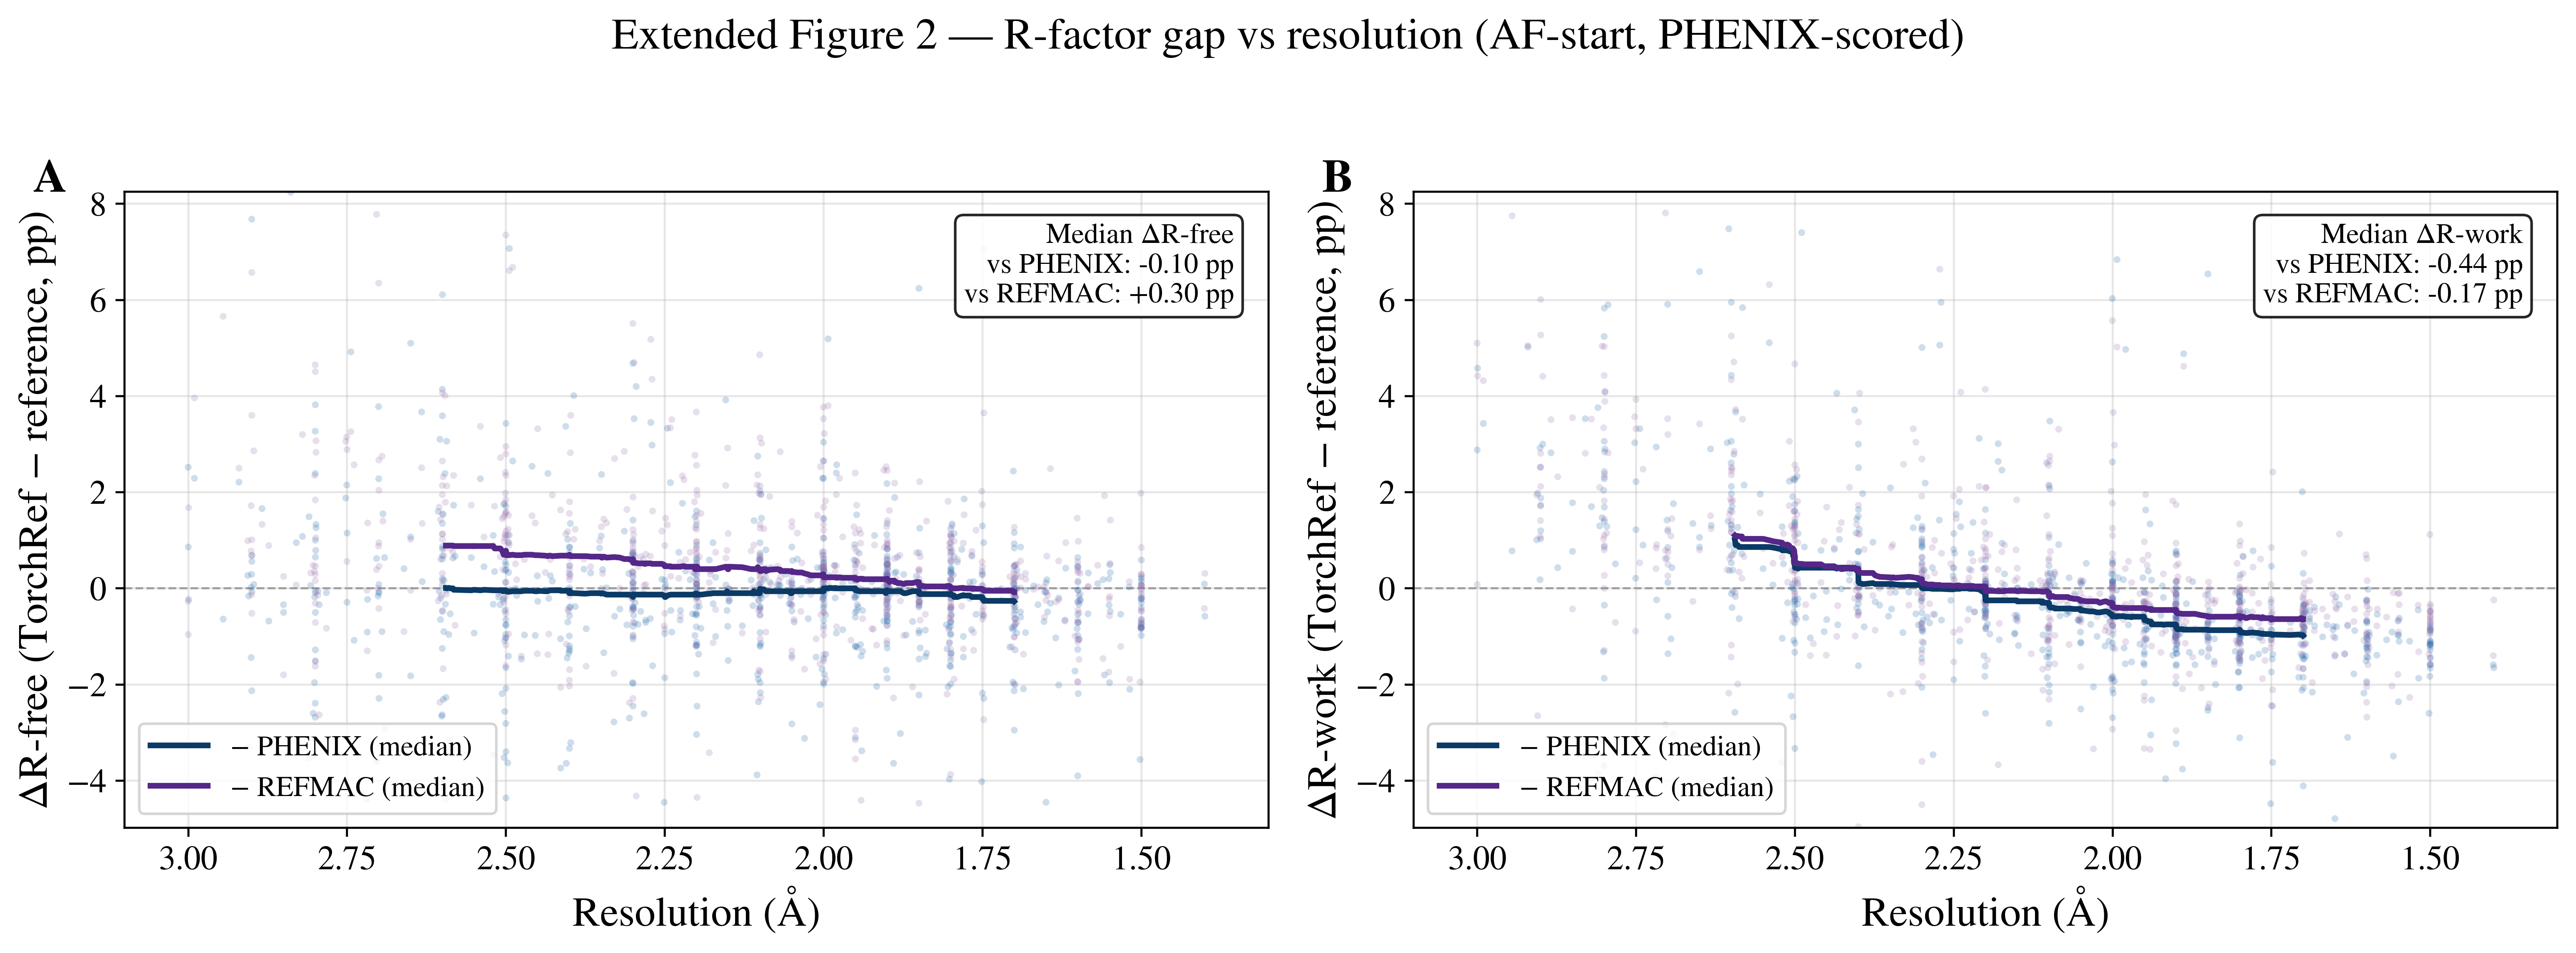
\includegraphics[width=\textwidth]{figS2.png}
\end{center}
\caption{%
  Per-structure TorchRef$-$reference R-factor differences as a function of
  resolution on the AlphaFold benchmark ($n = 725$ structures,
  $d_\mathrm{min}$ range $1.40$--$3.00$~\AA), with a light scatter and a
  bold running-median line for each reference program: Phenix (blue) and
  REFMAC5 (purple). A positive $\Delta R$ indicates that TorchRef's R-factor is higher than the reference.
  Panel A: $\Delta R_\mathrm{free}$ vs resolution.  Overall medians are
  $-0.10$~percentage points (pp) vs Phenix and $+0.30$~pp vs REFMAC5, consistent with the
  cross-engine $R_\mathrm{free}$ agreement reported in the main text.
  Panel B: $\Delta R_\mathrm{work}$ vs resolution. Overall medians are
    $-0.44$~pp vs Phenix and $-0.17$~pp vs REFMAC5.
}
\label{fig:figS2}
\end{figure}

\begin{figure}[ht]
\begin{center}
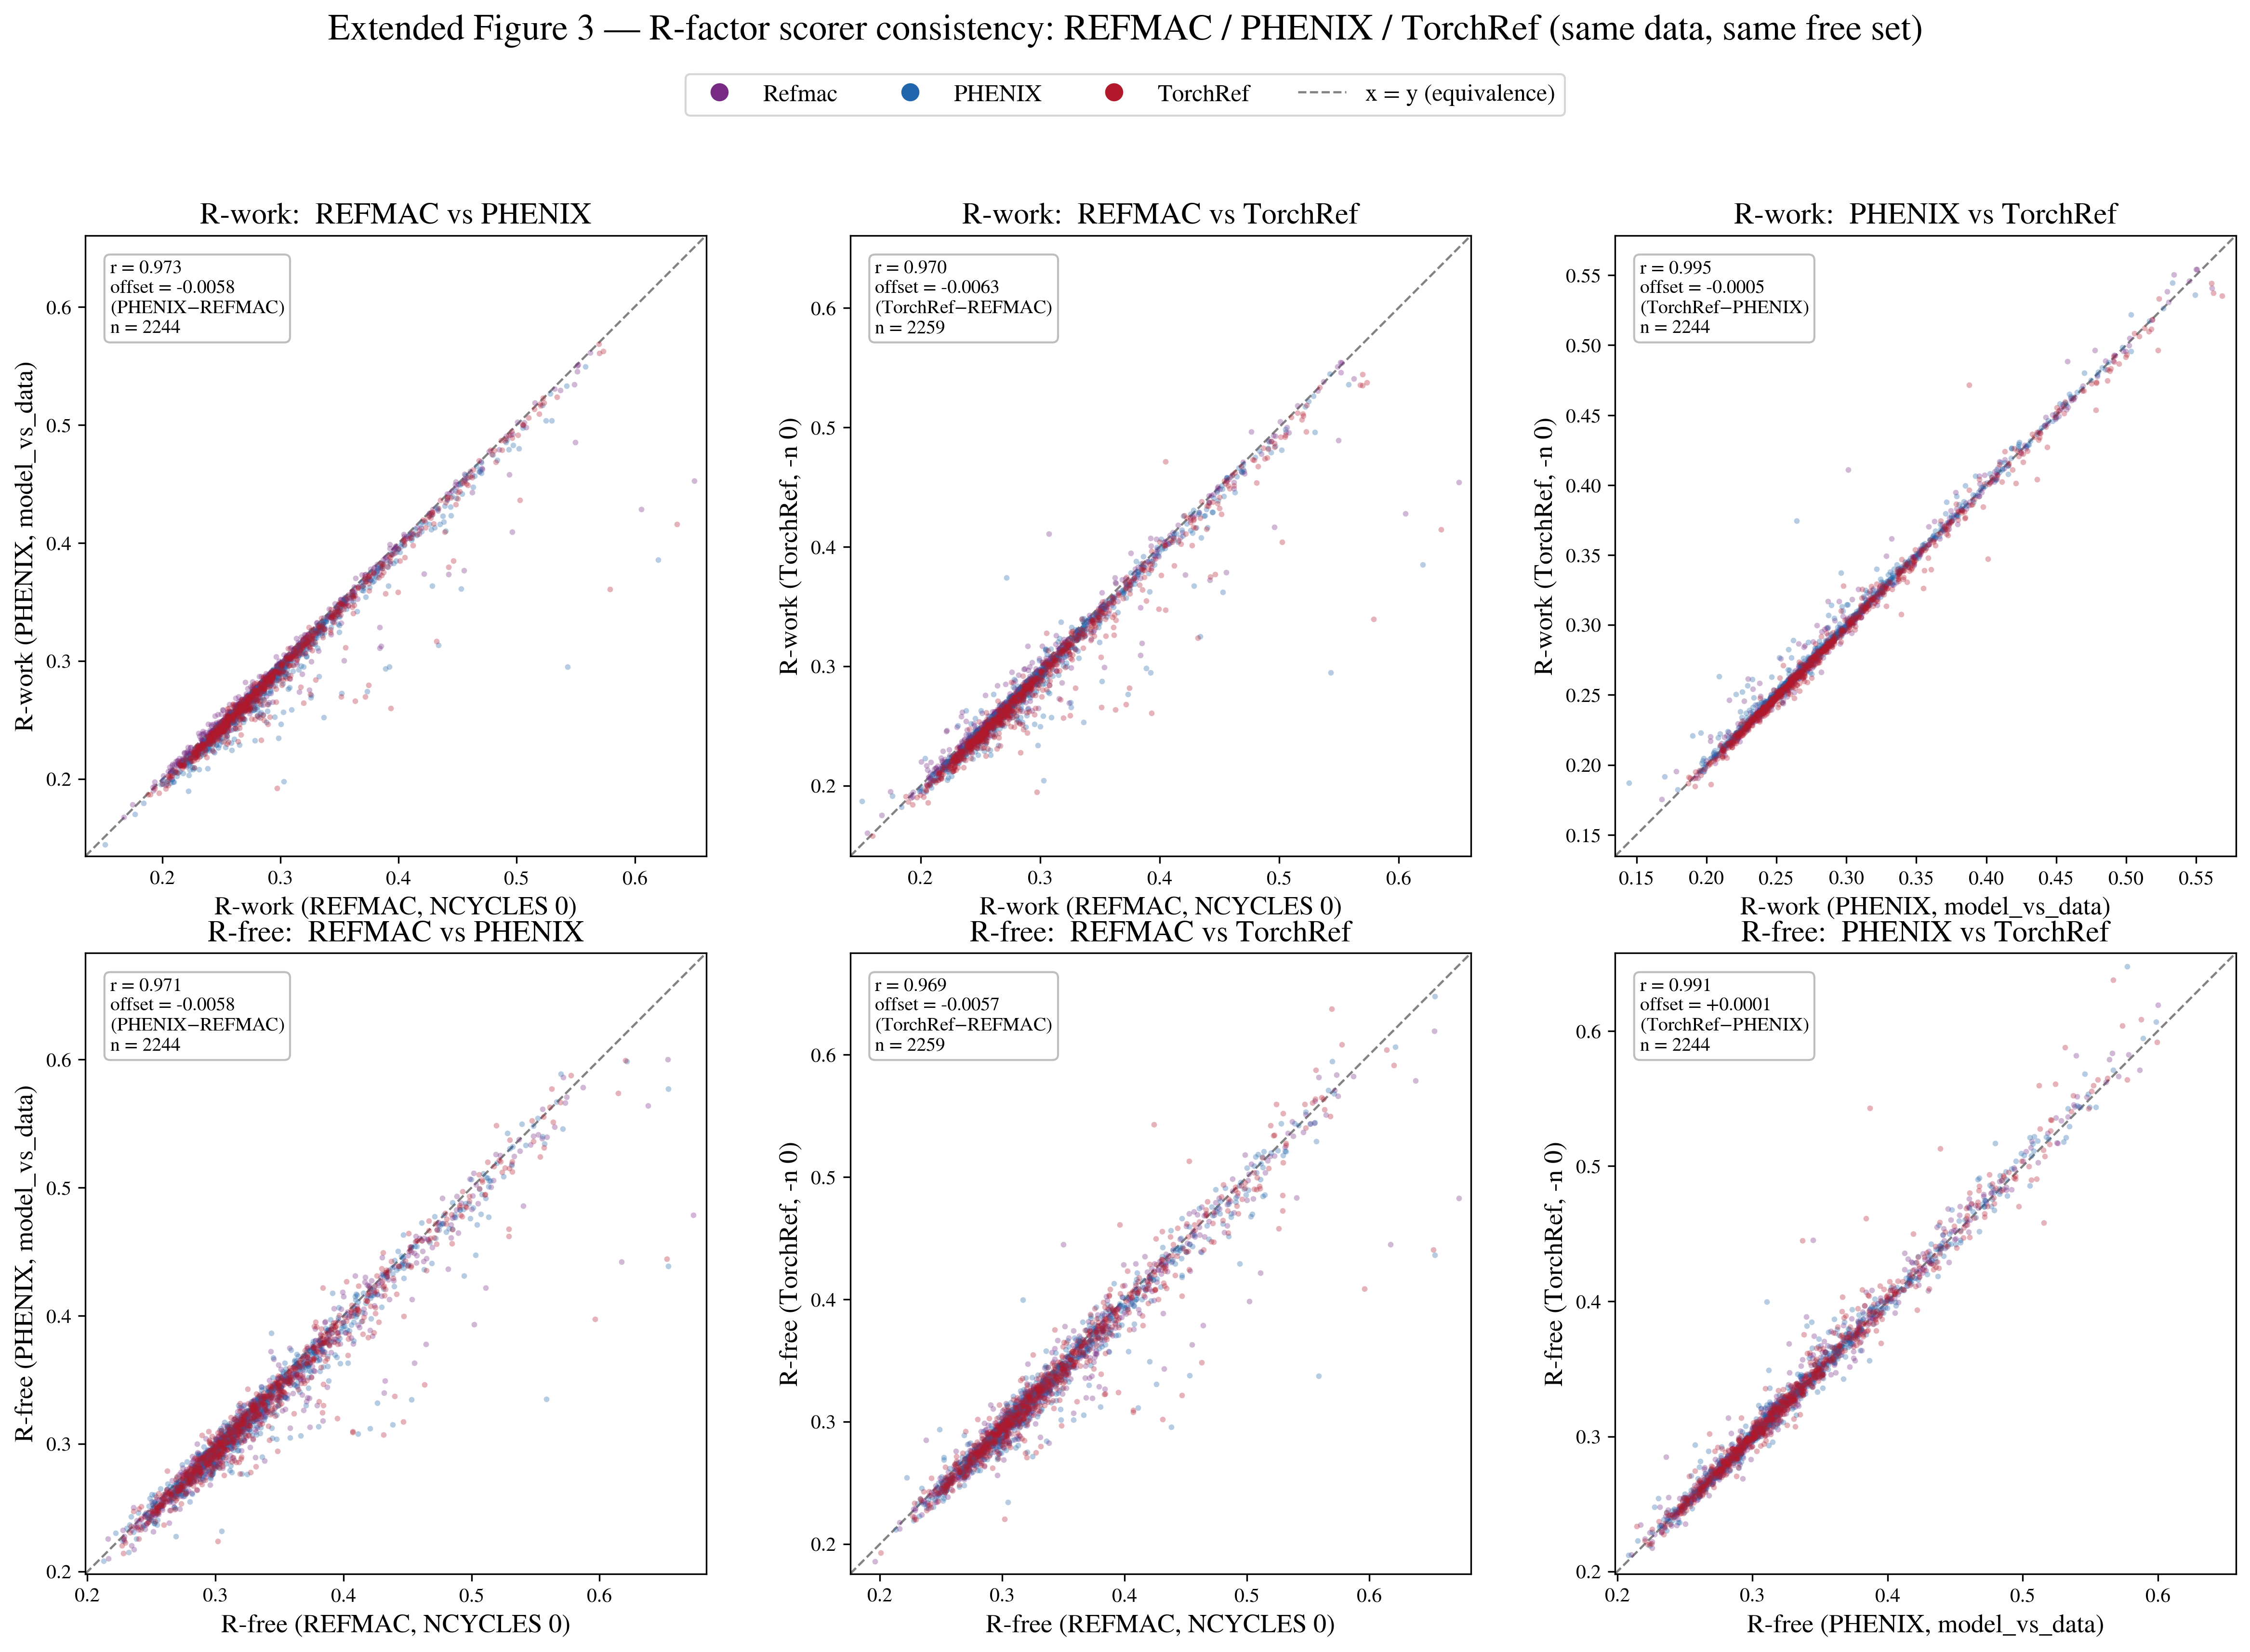
\includegraphics[width=\textwidth]{figS3.png}
\end{center}
\caption{%
  R-factor scorer cross-consistency on the AlphaFold benchmark.
  Every refined model (\texttt{refmac5}, \texttt{phenix.refine}, TorchRef; coloured
  by the engine that produced it) was independently re-scored against
  identical structure factors and free flags by three R-factor scorers
  operating in zero-cycle mode (scaling and bulk-solvent fit only;
  coordinates and ADPs untouched): REFMAC5 with \texttt{NCYCLES 0},
  \texttt{phenix.model\_vs\_data}, and \texttt{torchref.refine -n 0}.
  Top row: $R_\mathrm{work}$. Bottom row: $R_\mathrm{free}$. Each panel
  shows pairwise scatter between two scorers, with Pearson correlation $r$,
  signed median offset (scorer\textsubscript{y} $-$ scorer\textsubscript{x}),
  and sample count annotated. The dashed line is the equivalence diagonal
  $x = y$. Phenix and TorchRef show very close agreement
  ($r = 0.995$ for $R_\mathrm{work}$, $r = 0.991$ for $R_\mathrm{free}$),
  with signed median offsets of $-0.0005$ and $+0.0001$, respectively.
  REFMAC5 vs TorchRef gives $r = 0.970$ for $R_\mathrm{work}$ and
  $r = 0.969$ for $R_\mathrm{free}$, with median offsets of $-0.0063$ and
  $-0.0057$. REFMAC5 and Phenix give
  $r = 0.973$ for $R_\mathrm{work}$ and $r = 0.971$ for
  $R_\mathrm{free}$, with offsets of $-0.0058$ and $-0.0058$.
  The three scorers measure equivalent R-factors to within a small
  systematic offset across all engine pairings, supporting the choice of
  \texttt{phenix.model\_vs\_data} as the headline scorer in the main
  figure.}
\label{fig:figS3}
\end{figure}

\begin{figure}[ht]
\begin{center}
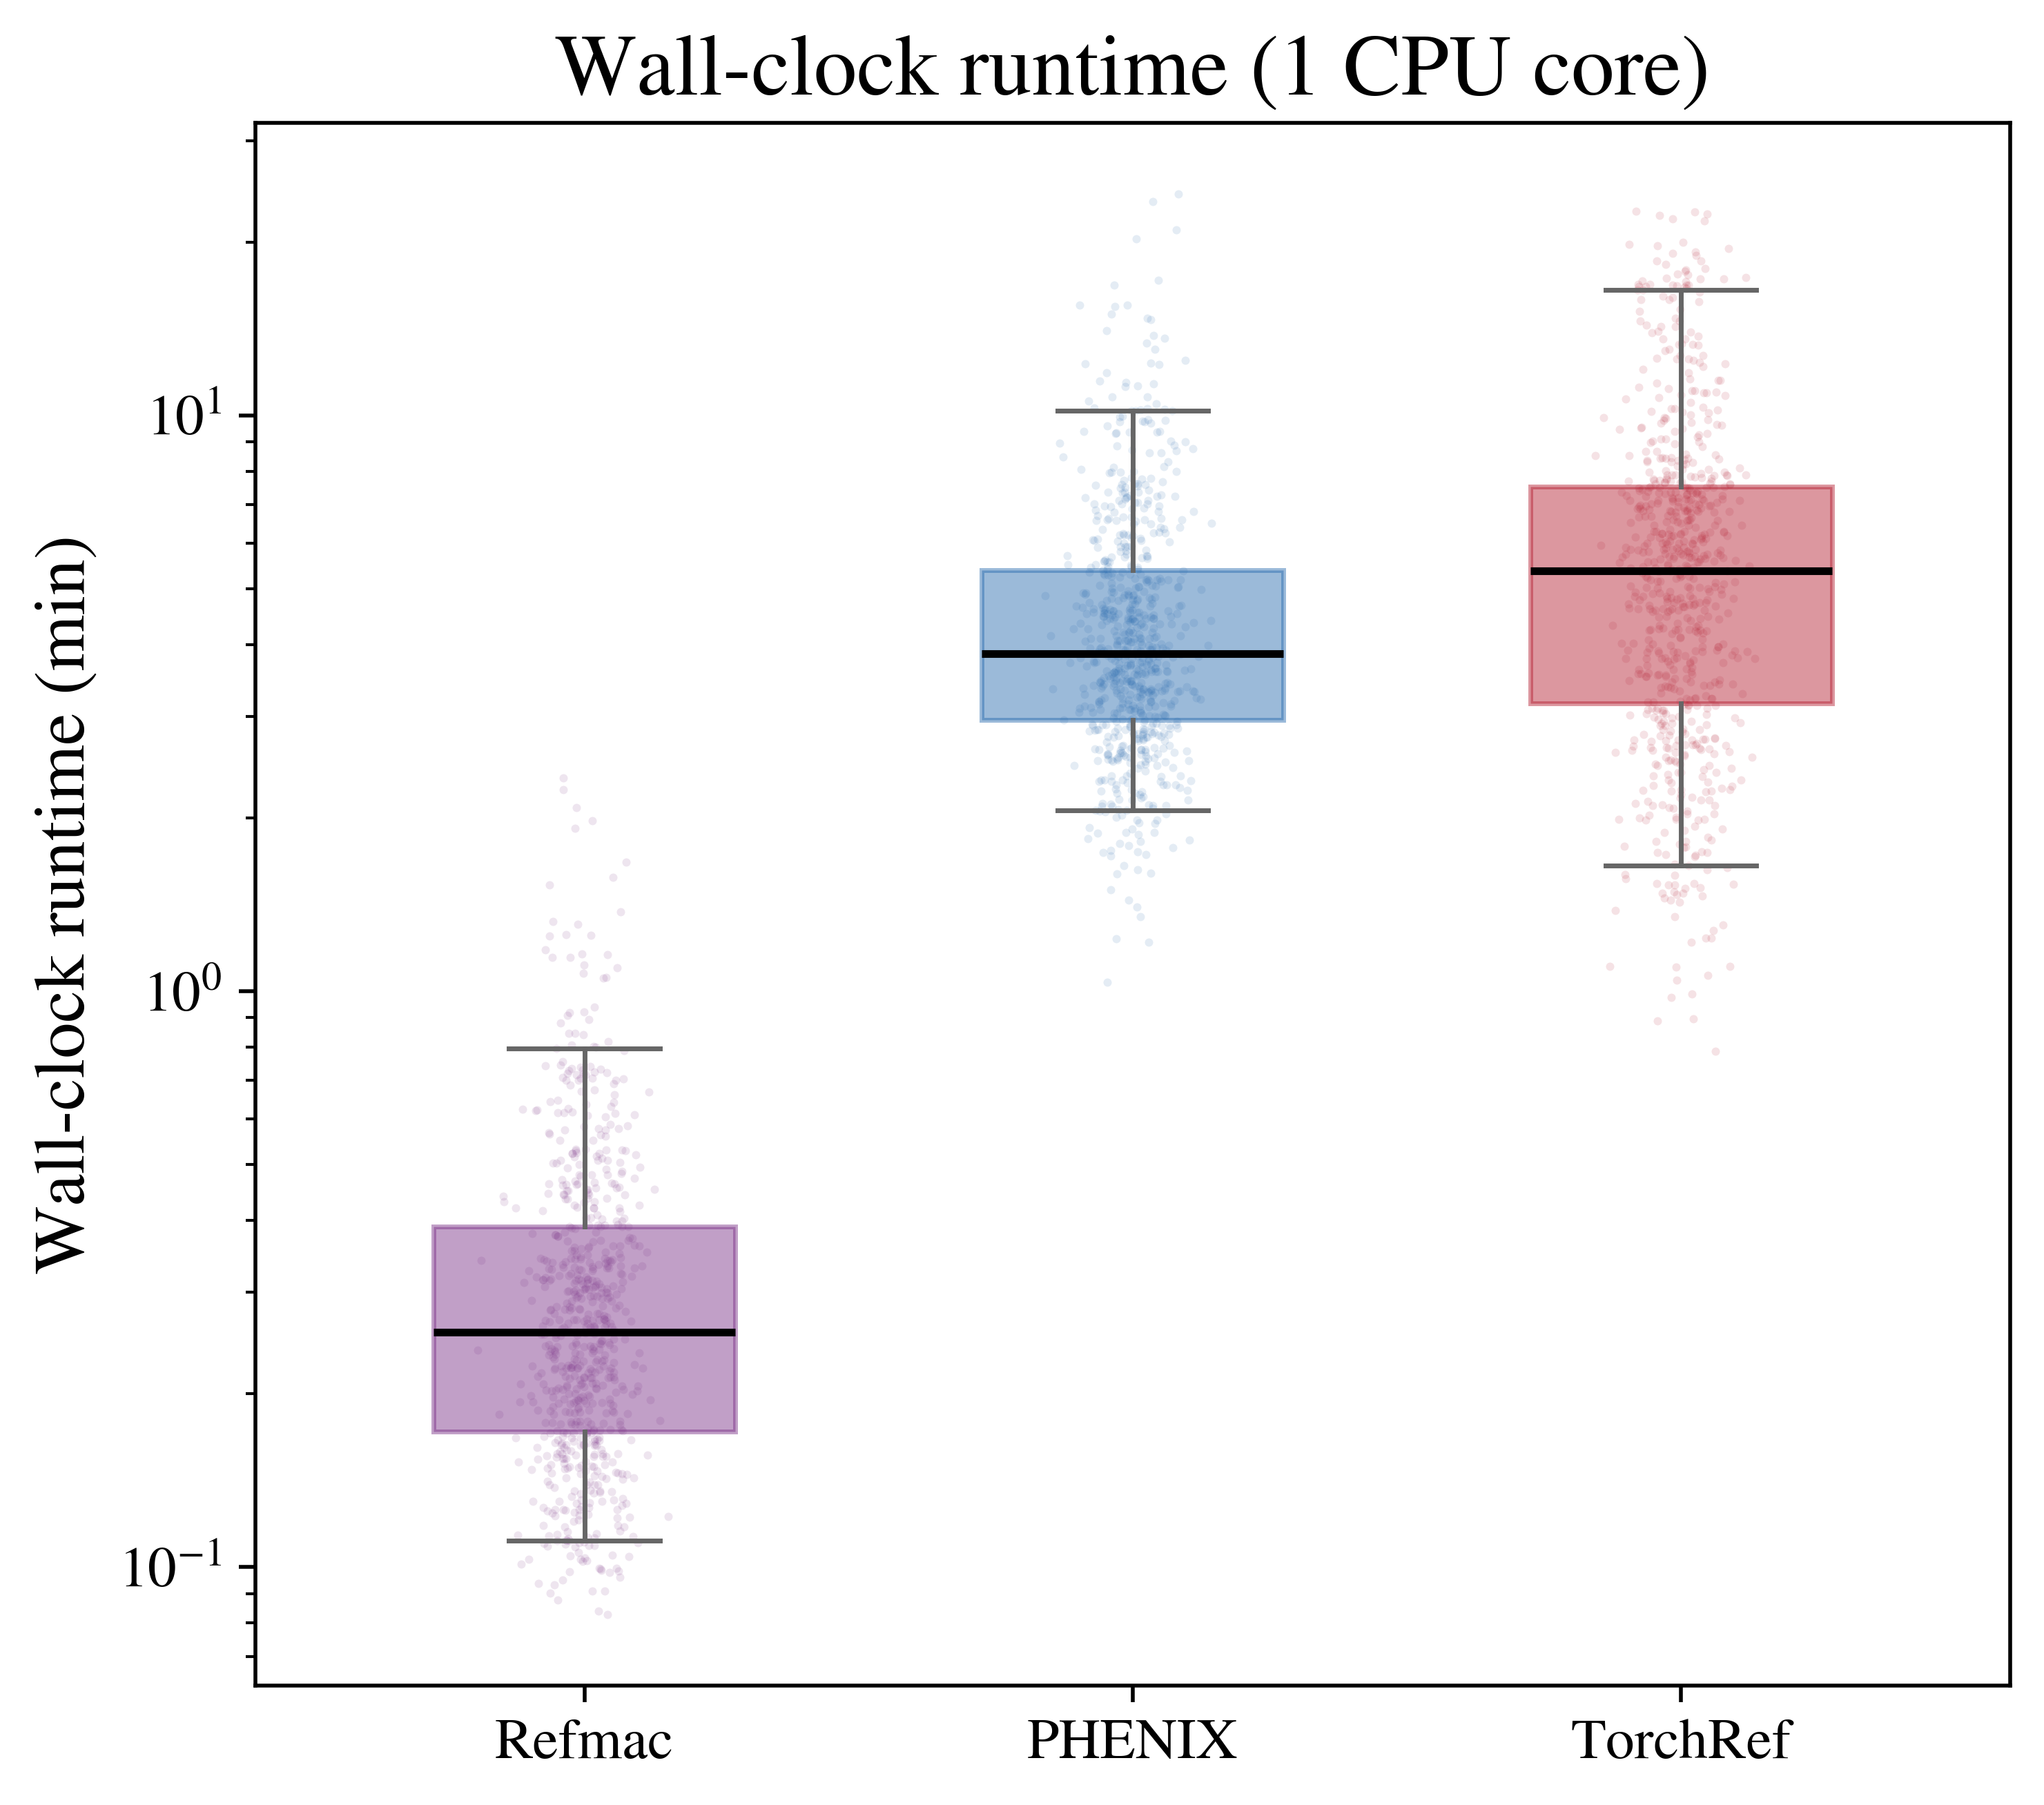
\includegraphics[width=\textwidth]{figS4.png}
\end{center}
\caption{%
  Single-core wall-clock runtime on the AlphaFold benchmark, with every
  engine pinned to a single CPU thread (TorchRef
  \texttt{TORCHREF\_NUM\_THREADS=1}; \texttt{phenix.refine}
  \texttt{refinement.main.nproc=1}; REFMAC5 with
  \texttt{OMP\_NUM\_THREADS=1}).  The same conserved cohort as in main-text
  Fig.~2C was re-timed at one core ($n = 723$). Box plots are 25--75th percentile with
  5--95th percentile whiskers; the faint jittered strip shows individual
  structures. Ratios of the engine medians show TorchRef is $\approx 21.0\xfac$ slower
  than REFMAC5 and $\approx 1.4\xfac$ slower than \texttt{phenix.refine}
  at one core; this contrasts with the four-core
  comparison in Fig.~2C, where TorchRef pulls clearly ahead of \texttt{phenix.refine}.
  TorchRef also shows a noticeably wider per-structure runtime
  distribution than \texttt{phenix.refine} and REFMAC5, with a long
  upper tail driven by the largest structures in the cohort.
  REFMAC5's single-core performance is essentially unchanged from its
  four-core performance because it does not use OpenMP parallelism.}
\label{fig:figS4}
\end{figure}

\clearpage


%==============================================================================
\section*{Supplementary methods}
%==============================================================================


%==============================================================================
\section{Scope and notation}
%==============================================================================

This document describes the quantities TorchRef refines, the structure factor
calculation, and the implemented target functions.
Where a default value is sourced from external data (e.g.\ the CCP4 monomer
library) and varies per restraint, this is noted explicitly.

Throughout, we use the following notation.
$F$ refers to the (complex) structure factor and $|F|$ the amplitude.
$F_{o}$ is the observed structure factor amplitude and
$F_{c} = |F_\mathrm{calc}|$ the model amplitude; $\sigma$ the experimental
uncertainty on $F_{o}$.
The scattering vector is $\mathbf{s}$ with
$s = |\mathbf{s}| = 2\sin\theta/\lambda$ (\AA$^{-1}$);
$d^\ast = 1/d = s$ and $d^{\ast 2}=1/d^2=s^2$;
$s_{1/2} = \sin\theta/\lambda = s/2$ (\AA$^{-1}$) is used when atomic form
factors are tabulated in the $(\sin\theta/\lambda)^{2}$ convention of the
\emph{International Tables for Crystallography}, Vol.~C (ITC92)
\cite{wilson_international_1992}.
The reflection multiplicity $\varepsilon$ is the number of rotational
symmetry operations mapping $\mathbf{h} \rightarrow \pm\mathbf{h}$,
including the inversion $\mathbf{h} \rightarrow -\mathbf{h}$.
This Friedel-aware convention differs from the classical Wilson
$\varepsilon$ (which counts only $R^{\mathsf{T}}\mathbf{h} = \mathbf{h}$) by
inclusion of inversion symmetry.
$B$ denotes an isotropic atomic displacement parameter (\AA$^{2}$) and
$\mathbf{U}$ an anisotropic ADP tensor (\AA$^{2}$).
For an isotropic atom $U_\mathrm{iso} = B/(8\pi^{2})$; the anisotropic
Debye--Waller factor uses
$\exp(-2\pi^{2}\mathbf{s}^{\mathsf{T}}\mathbf{U}\mathbf{s})$, where $\mathbf{s}$
is the Cartesian scattering vector (see Eq.~\ref{eq:dw-aniso}), with equivalent
isotropic $B_\mathrm{eq} = (8\pi^{2}/3)\,\mathrm{tr}(\mathbf{U})$.
$I_{0}, I_{1}$ are modified Bessel functions of the first kind, and
$\mathrm{i0e}(x) = e^{-x}I_{0}(x)$, $\mathrm{i1e}(x) = e^{-x}I_{1}(x)$ denote
their exponentially scaled forms, and
$\mathrm{logi0e}(x) = \log\mathrm{i0e}(x) = \log I_{0}(x) - x$ its logarithm.
We write $\mathbf{h}$ for a Miller-index triple; in reflection sums and
subscripts of the form $\sum_{h}$ or $w_{h}$, the symbol $h$ is the running
enumeration index over the flattened reflection list.

%==============================================================================
\section{Reflection data preparation}
%==============================================================================

Before refinement begins, observed intensities are converted to amplitudes,
reflections are flagged for cross-validation, and outliers and suspicious
uncertainties are masked.  All steps operate on a \texttt{ReflectionData}
object that stores reflections in the standard CCP4 asymmetric-unit (ASU)
convention, which all downstream HKL operations assume.

\subsection{Intensity-to-amplitude conversion (French--Wilson)}

When the input data are intensities $I$ with uncertainties $\sigma_{I}$,
TorchRef converts them to amplitudes via the French--Wilson treatment
\cite{french_treatment_1978}.  The implementation follows the \texttt{mmtbx}
French--Wilson routine, with separate centric and acentric
branches.

Reflections are first binned in equal-count resolution shells (60 bins,
minimum 40 reflections per bin).  The per-shell Wilson mean $\langle I \rangle$
is estimated on the available reflections in each shell, then linearly
interpolated in $d$-spacing to each reflection.  Given the French--Wilson
normalised intensity $h = I/\sigma_{I} - \sigma_{I}/\langle I \rangle$
(acentric; the centric branch uses $\sigma_{I}/2\langle I \rangle$ for the
second term), the conditional posterior mean and variance of $|F|$ are
evaluated and scaled by $\sqrt{\sigma_{I}}$.  Two regimes are used: a precomputed lookup table for
small $h$ (acentric $h<3$, centric $h<4$), and a closed-form asymptotic
expansion at large $h$ using the centric and acentric series.
%
Reflections with non-finite $I$ or $\sigma_{I}$ are filled with NaN and
excluded from downstream computation; strongly negative or very-low-$\sigma$
reflections within the standard French--Wilson regime are
\emph{not} excluded but have $h$ clamped to the boundary lookup value
$h_{\min} = -4.0$; a companion threshold $(I/\sigma)_{\min} = -3.7$ marks
the boundary of the separate boolean \texttt{valid\_mask}.  The per-shell
Wilson mean is recomputed on every forward pass, so the conversion tracks
updated intensities without re-preprocessing.

\subsection{Outlier and suspicious-$\sigma$ flagging}

All masking is model-free and applied once at data load: no calculated-amplitude
outlier rejection is performed.

\paragraph{Data-validity flagging.}
Reflections with a non-finite $F$ or $\sigma$, or a non-positive $F$, are dropped
(mask \texttt{sanity\_F}). Intensity inputs additionally pass the French--Wilson
input guard, which drops measurements too negative to be a noisy sample of any
non-negative true intensity, the case for which its posterior integral cannot be evaluated.
With $\langle I\rangle$ the mean intensity of the reflection's shell (estimated per
shell and interpolated in resolution), the guard keeps a reflection when
%
\begin{equation}
  h \;=\; \frac{I}{\sigma_{I}}
  - \frac{\sigma_{I}}{\varepsilon_\mathrm{W}\,\langle I\rangle}
  \;\ge\; -4,
  \qquad
  \varepsilon_\mathrm{W} =
  \begin{cases} 2 & \text{centric,}\\ 1 & \text{acentric,}\end{cases}
  \label{eq:fw-h}
\end{equation}
%
(together with $I/\sigma_{I} \ge -3.7$), $h$ being the argument of the Wilson prior
folded with Gaussian measurement error, the centric case carrying twice the prior
variance. This is a validity guard on the intensity-to-amplitude conversion,
distinct from the outlier test below.

\paragraph{Wilson-outlier flagging.}
The outlier test is model-free (it never sees an $F_\mathrm{calc}$) and asks
how improbable each observation is under Wilson statistics for its resolution
shell, multiplicity and centricity, in \emph{both} tails. Its reference is the
Wilson scale $S = \varepsilon_\mathrm{W}\,\Sigma$ (the expected intensity), where $\Sigma$ is estimated
from the data as a robust per-shell median (the median of $\mathrm{Exp}(1)$ is
$\ln 2$ and of $\chi^{2}_{1}$ is $0.4549$, converting a shell median back to
$\Sigma$ with no fit), taken separately for centric and acentric reflections,
scaled by the reflection multiplicity, and given an anisotropic correction
$\Sigma_\mathrm{iso}(d)\,\exp(-2\pi^{2}\,\mathbf{s}^{\top}\mathbf{U}\,\mathbf{s})$
fitted to the observations: the median stops a strong outlier from inflating its
own reference, and the anisotropy stops an isotropic $\Sigma$ from flagging the
strong reciprocal direction of every anisotropic dataset. Convolving the Wilson
prior with the Gaussian measurement error gives a predictive density whose upper
tail is closed form,
%
\begin{equation}
  P(I' > I) \;=\; Q\!\left(\tfrac{I}{\sigma_{I}}\right)
  + \exp\!\left(\frac{\sigma_{I}^{2}}{2 S^{2}} - \frac{I}{S}\right)
    \Phi\!\left(\tfrac{I}{\sigma_{I}} - \tfrac{\sigma_{I}}{S}\right),
  \qquad Q = 1 - \Phi ,
  \label{eq:wilson-outlier}
\end{equation}
%
whose $\Phi$ argument is the statistic of Eq.~\ref{eq:fw-h} evaluated against this
robust $S$; the closed form is exact for acentric reflections, with centrics
handled by the same expression under the French--Wilson factor-of-two convention
($S = 2\Sigma$), which captures the correct tail exponent. A reflection is rejected
when it sits further into the strong tail
($\log P(I'>I)$ below threshold: zingers, ice rings, mis-integrated spots) or the
weak tail ($h$ below threshold) than the dataset size can account for: the
threshold is a family-wise error rate $\alpha/N$ over the $N$ tested reflections
(default $\alpha = 0.01$), so it tightens as the dataset grows rather than rejecting
a fixed fraction. Only reflections finer than $4$~\AA{} are tested, where bulk
solvent no longer dominates and the shells are well populated, and $\Sigma$ and
$\mathbf{U}$ are refit in a second pass with the first pass's outliers held out.
Amplitude-only inputs reconstruct intensities ($I = F^{2}$,
$\sigma_{I} = 2F\sigma_{F}$) first; the negative tail is then blind (the amplitude
is a positive posterior mean) but the strong tail, where outliers sit, is
unaffected.

\paragraph{Suspicious-$\sigma$ flagging.}
A secondary, diagnostic-only pass, superseded in the automatic load path by the
Wilson test above.  Reflections with non-finite $\sigma$, and those whose
$\log\sigma$ lies more than $z = 5$ standard deviations from the bulk
distribution, are flagged (mask \texttt{flagged\_sigma}); the standard deviation is
stabilised with a small term proportional to the mean
($10^{-5}\langle\log\sigma\rangle$).


\subsection{Cross-validation flags}

TorchRef supports a three-way \emph{work / free / validation} partition of
the reflections. The work and free sets follow the cross-validation recipe
of \cite{brunger_rfree_1992}: free reflections do not contribute direct
coordinate or ADP gradients and serve two roles. First, they provide the
reference for the $R_\mathrm{free}$ profile. Second, they are the sample from
which the model-error component $\beta_\mathrm{model}$ and total variance $\beta$ of the
$\sigma_{A}$ maximum-likelihood target (see \emph{X-ray target functions
$\to$ Maximum-likelihood $\sigma_{A}$ target} below) are
derived, via a maximum-likelihood estimate of $\sigma_A$, using noise-corrected
moments on equal-count free-set shells. Because this detached error model uses
the free reflections, $R_\mathrm{free}$ is a useful profile diagnostic but not
a strictly untouched held-out score.

R-free flags are assigned by resolution-stratified sampling: equal-count
shells ordered in $d^{\ast2}$ (10 bins, minimum 1000 reflections per bin) with a target
free fraction of $2\%$ per bin.  A separate per-bin floor of $50$
free reflections (clamped to the bin size on tiny bins) keeps the
per-shell statistics usable for small datasets.  The draw is over unique
CCP4-asymmetric-unit reflections rather than over rows: the two members of a
Bijvoet pair share a canonical ASU index and are assigned the same flag, so
Friedel mates are never split across the work/free boundary.  

The optional \emph{validation set} is a disjoint third subset carved from
the free set on request (default: half of the free reflections), using the
same resolution-stratified sampler and stored in a separate boolean
\texttt{validation\_flags} buffer that survives MTZ round-trip; the binary
R-free flags are unchanged.  Standard refinement does not use it: the
optimisation uses the work set and $R_\mathrm{free}$ is reported against the
free set as usual.  The validation set supports tuning choices outside the
likelihood (model size, regularisation strength, ensemble size) without
contaminating the free-set statistic.



%==============================================================================
\section{Parameterisation}
%==============================================================================

A central design choice of TorchRef is to map atomic displacement parameters
(ADPs) and occupancies to unconstrained latent parameters through an invertible
transform: a $\log$ map for the isotropic $B$, a Cholesky factor for the
anisotropic $\mathbf{U}$, and a logit for the occupancy.
The mapping enforces the physical parameter bounds explicitly: negative $B$,
indefinite $\mathbf{U}$ and occupancy outside $[0,1]$ are impossible by
construction, so an unconstrained optimiser can act on every parameter type
without bound constraints. The production schedule retains the tested blockwise
protocol, alternating scaler, xyz, and ADP/occupancy blocks per
macrocycle (see \emph{Macrocycle structure} below).
All gradients with respect to the latent variables are obtained by automatic
differentiation.
Each parameterisation below is an independent PyTorch module behind a uniform
interface, so any can be swapped for a user-defined alternative without touching
the rest of the pipeline.

\subsection{Coordinates}

Atomic coordinates are parameterised in Cartesian space,
$\mathbf{x}_\mathrm{cart} \in \mathbb{R}^{N \times 3}$ (\AA).
Fractional coordinates are derived on demand from the orthogonalisation matrix
$\mathbf{O}$ via Eq.~\ref{eq:frac-cart}:
%
\begin{equation}
  \mathbf{x}_\mathrm{frac} = \mathbf{x}_\mathrm{cart}\,\mathbf{O}^{-\mathsf{T}},
  \qquad
  \mathbf{x}_\mathrm{cart} = \mathbf{x}_\mathrm{frac}\,\mathbf{O}^{\mathsf{T}}.
  \label{eq:frac-cart}
\end{equation}
%
Internal/torsion-angle parameterisations have been investigated in the past but
have since been deprecated.

\subsection{Atomic displacement parameters}

\textbf{Isotropic} $B$-values are refined in log-space, guaranteeing positivity
for any real latent $p$ (Eq.~\ref{eq:adp-iso}):
%
\begin{equation}
  B = \exp(p), \qquad p = \log(\max(B,\epsilon)),
  \qquad \epsilon = 0.1~\text{\AA}^{2}.
  \label{eq:adp-iso}
\end{equation}
%
\textbf{Anisotropic} ADPs are parameterised through a Cholesky factor
$\mathbf{U} = \mathbf{L}\mathbf{L}^{\mathsf{T}}$ with six free parameters, which
keeps $\mathbf{U}$ positive-definite by construction, with $\mathbf{L}$ as in
Eq.~\ref{eq:adp-aniso-chol}:
%
\begin{equation}
  \mathbf{L} =
  \begin{pmatrix}
    \exp(p_{0}) + \epsilon & 0 & 0 \\
    p_{3} & \exp(p_{1}) + \epsilon & 0 \\
    p_{4} & p_{5} & \exp(p_{2}) + \epsilon
  \end{pmatrix},
  \qquad \epsilon \text{ a small positive floor}.
  \label{eq:adp-aniso-chol}
\end{equation}
%
The decomposition is performed only at initialisation (and on freeze/unfreeze),
never inside the forward loop, so the optimiser can never drive $\mathbf{U}$
indefinite and produce NaNs in the structure factor FFT.

\subsection{Occupancies}

Occupancies are refined through a logit/sigmoid map (Eq.~\ref{eq:occ-sigm}),
%
\begin{equation}
  \mathrm{occ} = \mathrm{sigm}(p) = \frac{1}{1 + e^{-p}},
  \label{eq:occ-sigm}
\end{equation}
%
with initial values clamped just inside $[0,1]$.
Shared sites collapse to a single latent via an expansion mask.
Linked occupancies (e.g.\ alternative conformations that must sum to unity
within an alt-conf group) are enforced by parameterisation: the effective
occupancy entering the structure factor calculation is the group-normalised
sigmoid of the logit, as in Eq.~\ref{eq:occ-link}.
%
\begin{equation}
  \mathrm{occ}_{i} \;=\;
  \frac{\mathrm{sigm}(p_{i})}{\sum_{j \in \mathrm{group}} \mathrm{sigm}(p_{j})}.
  \label{eq:occ-link}
\end{equation}


\subsection{Refinable / fixed parameter split}

Each refinable parameter type keeps the full atom set as a frozen buffer and
an index that maps the currently-refinable subset into it.  The full
parameter array is reconstructed at every forward pass by scattering the
refinable subset into that buffer; freezing or unfreezing a selection
rebuilds the index.

\subsection{ADP-mode switching at runtime}\label{sec:adp-mode}

Atomic displacement parameters can be switched between isotropic and
anisotropic storage at runtime, without rebuilding the model.  A mixed
isotropic $+$ anisotropic representation is realised by a per-atom
\texttt{mmtbx}-style selection string (default:
\texttt{"not resname HOH and not element H"}) that marks the atoms
carrying anisotropic ADPs.  The conversion math:
%
\begin{itemize}
\item Anisotropic $\rightarrow$ isotropic: the equivalent isotropic
  $B$-value is taken as the standard equivalent of the diagonal trace,
  $B_\mathrm{eq} = (8\pi^{2}/3)\,\mathrm{tr}(\mathbf{U})$.
\item Isotropic $\rightarrow$ anisotropic: the isotropic $B$ is broadened
  into a diagonal $\mathbf{U}$ with $U_\mathrm{iso} = B/(8\pi^{2})$ and
  zero off-diagonal components.  The Cholesky parameterisation (see
  ``Anisotropic ADPs'' above) is rebuilt from the new $\mathbf{U}$.
\end{itemize}
%
The repartition updates all downstream caches (structure factor indexing,
refinable masks, and PDB anisotropy flags); it is a full repartition, not a
value-only conversion.


%==============================================================================
\section{Structure factor calculation}
%==============================================================================

TorchRef provides two structure factor back-ends: a direct (Debye) summation
and an FFT-based path, the latter being the default for production refinement.
The sign convention is $\exp(+2\pi i\,\mathbf{h}\cdot\mathbf{r})$.

\subsection{Reciprocal basis and late symmetry expansion}

The reciprocal basis is built from the cell parameters
$(a,b,c,\alpha,\beta,\gamma)$ in a lower-triangular real-space convention,
as in Eq.~\ref{eq:reciprocal-basis},
%
\begin{equation}
  \mathbf{a}^{*} = \frac{\mathbf{b}\times\mathbf{c}}{V},\quad
  \mathbf{b}^{*} = \frac{\mathbf{c}\times\mathbf{a}}{V},\quad
  \mathbf{c}^{*} = \frac{\mathbf{a}\times\mathbf{b}}{V},\quad
  V = \mathbf{a}\cdot(\mathbf{b}\times\mathbf{c}),
  \label{eq:reciprocal-basis}
\end{equation}
%
with $\mathbf{s} = h\,\mathbf{a}^{*} + k\,\mathbf{b}^{*} + l\,\mathbf{c}^{*}$.

The density and FFT are computed in space group $P1$, and crystal symmetry is
applied in reciprocal space (Eq.~\ref{eq:sym-expansion}), which is exact on
the integer grid and avoids expanding symmetry-related copies of every atom,
%
\begin{equation}
  F_\mathrm{sym}(\mathbf{h}) = \sum_\mathrm{ops}
  \exp\!\left(2\pi i\,\mathbf{h}\cdot\mathbf{t}_\mathrm{op}\right)
  F_{P1}\!\left(\mathbf{R}_\mathrm{op}^{\mathsf{T}}\mathbf{h}\right).
  \label{eq:sym-expansion}
\end{equation}

The grid is chosen to be compatible with the space group, and optimised to be FFT-friendly.

Reflections are canonicalised to the CCP4 asymmetric unit by
\texttt{gemmi.ReciprocalAsu}, via a vectorised fast path that covers the
ten distinct CCP4 ASU conditions (sufficient for all 230 space groups
\cite{agirre_ccp4_2023, wojdyr_gemmi_2022}).  Canonicalisation also
applies the phase correction
$\varphi_\mathrm{new} = \varphi_\mathrm{old} + \varphi_\mathrm{shift}$,
with a sign flip on Friedel mates, so that ASU-stored amplitudes and
phases remain consistent with the unit-cell origin.

\subsection{Atomic scattering factors}

Atomic form factors use the ITC92 parameterisation, which is a sum of
four Gaussians plus a constant
\cite{wilson_international_1992} as in Eq.~\ref{eq:itc92-form-factor},
%
\begin{equation}
  f(s) = \sum_{i=1}^{4} a_{i}\,\exp\!\left(-b_{i}\,s^{2}/4\right) + c.
  \label{eq:itc92-form-factor}
\end{equation}
%
For vectorisation, TorchRef packs the constant $c$ as a fifth Gaussian
($a_{5} = c$, $b_{5} = 0$), so evaluation is a single
$(N_{\mathrm{atoms}}, 5)$ contraction.

The form factors are shared by both structure factor back-ends: a Z-based
lookup against a precomputed table of neutral atoms ($Z = 1\ldots103$) yields
the $(N_{\mathrm{atoms}}, 5)$ coefficient tensors $\mathbf{A}$ and
$\mathbf{B}$.  The production path uses the neutral form factor regardless of
the input PDB's formal-charge column; ion-specific entries are available only
through an explicit helper.

\subsection{FFT path and electron-density sampling}

In the FFT path the model electron density is sampled onto a real-space grid
with spacing $d_\mathrm{min}/3$, and structure factors are
obtained by an inverse FFT, as in Eq.~\ref{eq:fc-fft},
%
\begin{equation}
  F(\mathbf{h}) = \frac{V_\mathrm{cell}}{N_\mathrm{voxels}}\,\mathrm{ifftn}(\rho),
  \label{eq:fc-fft}
\end{equation}
%
where \texttt{ifftn} denotes the un-normalised inverse FFT
(\texttt{torch.fft.ifftn(..., norm="forward")}); the prefactor
$V_\mathrm{cell}/N_\mathrm{voxels}$ is the voxel volume that converts the
discrete sum into the continuum integral, yielding complex structure factors
on the absolute scale.

Each atom's density is a sum of 3D Gaussians (one per scattering term) centred
on the atomic position. TorchRef truncates it at a per-atom radius large enough
to sample the atom's widest Gaussian out to $N_{\sigma}$ standard deviations
(default $N_{\sigma} = 3$), rounded up to the nearest $0.25$~\AA{} and clamped
to $[2, 7]$~\AA{}:
%
\begin{equation}
  r_\mathrm{atom} = \mathrm{clamp}\!\bigl(
    \mathrm{ceil}_{0.25}(N_{\sigma}\,\sigma_\mathrm{eff}),\;
    [2.0,\,7.0]~\text{\AA}
  \bigr),
  \label{eq:per-atom-radius}
\end{equation}
%
where $\sigma_\mathrm{eff} = \sqrt{(b_\mathrm{form} + B)/(8\pi^{2})}$ is the
effective real-space width built from the broadest ITC92 Gaussian width
$b_\mathrm{form}$ and the isotropic ADP $B$; anisotropic atoms use the largest
principal axis of the ADP tensor,
$\sigma_\mathrm{eff}^{2} = b_\mathrm{form}/(8\pi^{2}) + \lambda_\mathrm{max}(\mathbf{U})$.
Expressing the cutoff in sigmas gives every atom the same fractional Gaussian
tail, so the truncation residual is set by the single knob $N_{\sigma}$ rather than
by the worst atom; the default $N_{\sigma} = 3$ was validated against the
direct-summation reference.

The two device paths implement this per-atom radius differently. The CPU
sampler buckets atoms by box radius so that same-size atoms share a single
voxel loop.  The GPU path runs one Triton program per atom, each sizing its
bounding box from $r_\mathrm{atom}$ and truncating to the per-atom sphere
$r^{2}\!\leq\!r_\mathrm{atom}^{2}$.

TorchRef exploits the separability of a Gaussian on an orthogonal grid.
Writing the local coordinate offset as $(\delta x, \delta y, \delta z)$ along
the three orthogonal Cartesian axes, an isotropic Gaussian of width $w$
factorises as in Eq.~\ref{eq:gaussian-separable},
%
\begin{equation}
  \exp\!\left(-\frac{\delta x^{2} + \delta y^{2} + \delta z^{2}}{2w^{2}}\right)
  = \exp\!\left(-\frac{\delta x^{2}}{2w^{2}}\right)
    \exp\!\left(-\frac{\delta y^{2}}{2w^{2}}\right)
    \exp\!\left(-\frac{\delta z^{2}}{2w^{2}}\right),
  \label{eq:gaussian-separable}
\end{equation}
%
so the 3D contribution is the outer product of three 1D profiles.
For an orthogonal cell this reduces the per-atom cost from a naive
$(2R+1)^{3}$ exponential evaluations to $3(2R+1)$ per Gaussian term.
For monoclinic and hexagonal cells, exactly one pair of axes is oblique, so
the density factorises into one 1D profile along the orthogonal axis times
a 2D correction evaluated on the oblique plane, at a per-atom cost of
$(2R+1) + (2R+1)^{2}$ evaluations per term.
For triclinic cells, or for anisotropic scattering where no axis decouples,
TorchRef falls back to the full 3D evaluation.

The FFT path is validated against the eager direct-summation reference
using cosine-similarity and gradient-norm-ratio metrics on a scalar loss.

\subsection{Direct summation}

For isotropic ADPs, the structure factor is computed by direct summation as
in Eq.~\ref{eq:fc-direct},
%
\begin{equation}
  F(\mathbf{h}) = \sum_{j} \mathrm{occ}_{j}\, f_{0,j}(s)\,
  \exp\!\left(-B_{j}\, s^{2}/4\right)
  \exp\!\left(2\pi i\,\mathbf{h}\cdot\mathbf{x}_{j}\right),
  \label{eq:fc-direct}
\end{equation}
%
with $\mathbf{x}_{j}$ the fractional position of atom $j$ (so
$\mathbf{h}\cdot\mathbf{x}_{j}$ is dimensionless), using the thermally
attenuated neutral form factor $f_{0,j}(s)$. The anomalous contribution is
not part of this summation; as on the FFT path, it is added as a separate
post-processing step on the backend structure-factor output, as described in
Section~\ref{sec:anomalous} (in the current release wired only to the FFT
path). For atoms refined with anisotropic ADPs, the
isotropic Debye--Waller factor $\exp(-B_{j}s^{2}/4)$ in
Eq.~\ref{eq:fc-direct} is replaced atom-wise by the anisotropic form
in Eq.~\ref{eq:dw-aniso}; a mixed model with both iso- and aniso-refined
atoms is the sum of the two corresponding sub-sums,
%
\begin{equation}
  \exp\!\left(-2\pi^{2}\,\mathbf{s}^{\mathsf{T}}\mathbf{U}_{j}\,\mathbf{s}\right).
  \label{eq:dw-aniso}
\end{equation}
%
Summation is auto-batched and checkpointed over reflections to respect the
memory budget.  The eager direct-summation forward serves as the autograd
reference for the structure factor calculation; the GPU Triton kernels and
the gradient-checkpointed CPU path are validated against it.

\subsection{Anomalous scattering}\label{sec:anomalous}

The dispersive correction $f'$ is applied whenever the model contains
significant anomalous scatterers, and preserves Friedel's law; the absorptive
term $f''$, which breaks Friedel's law and produces Bijvoet differences, is
included only when the reflection data are loaded as unmerged Friedel pairs.
The atomic form factor is augmented with the dispersive and absorptive
corrections of Eq.~\ref{eq:anomalous},
%
\begin{equation}
  f(s, \lambda) \;=\; f_{0}(s) + f'(\lambda) + i\,f''(\lambda),
  \label{eq:anomalous}
\end{equation}
%
with $f'$ and $f''$ obtained per element from the Cromer--Liberman
calculation \cite{cromer_anomalous_1981} via \texttt{gemmi}, evaluated at the
model wavelength (default $1$~\AA{}).  The lookup is wavelength-dependent and
per-element but does not modulate with resolution; energy is converted from the
wavelength using $E_\mathrm{eV} = hc / \lambda$.

For per-step efficiency only elements with non-negligible $|f'|$ or
$|f''|$ (default threshold $0.5\,e$) contribute.  Light atoms (C, N, O, H)
are automatically filtered out at this stage; per-element correction values
and atom-index tensors are cached on the model.

The anomalous-correction cache is keyed on the model's element list, which
fixes $f'(\lambda)$ and $f''(\lambda)$ at the construction wavelength, and is
rebuilt when that list changes (e.g.\ after adding or removing heavy atoms);
a wavelength change requires an explicit cache reset.

No Debye--Waller term is applied to the anomalous heavy-atom
contribution; for floppy heavy atoms at high resolution, this is a
known approximation.

\subsection{Bulk-solvent mask}

The bulk-solvent mask is built in an \texttt{mmtbx}-style three-step procedure
\cite{afonine_robust_2005}: (i) atom-centred dilation by the
van~der~Waals radius of each heavy atom plus a probe radius
$R_\mathrm{probe}$ (default $1.1$~\AA{}); (ii) symmetry expansion of the
ASU mask to $P1$ on the density grid; (iii) erosion by a shrinkage
radius $R_\mathrm{shrink}$ (default $0.9$~\AA{}), implemented as a
solvent-side dilation followed by intersection with the mask
complement.  All distances respect the periodic boundary via the
minimum-image rule in fractional coordinates, which handles atoms that
straddle cell faces.

$F_\mathrm{mask}(\mathbf{h})$ is obtained from a single inverse FFT of the binary
solvent mask and scaled (Eq.~\ref{eq:scaling-components}) to produce the
bulk-solvent contribution $F_\mathrm{sol}(\mathbf{h})$.

The solvent parameters $\log k_\mathrm{sol}$, the falloff half-point
$\log s_{h}^{2}$ and sharpness $\log n$, and an optional phase offset
$\varphi_\mathrm{offset}$ are \texttt{nn.Parameter}s on the solvent module and are
refined alongside the other scaling parameters (Section~\ref{sec:scaling}).
The default scale follows Afonine \emph{et al.\/} ($k_\mathrm{sol} = 0.35$); the
falloff defaults to $n = 5$, so the solvent term switches off sharply near the
half-point rather than as a Debye--Waller factor (the $n = 1$ special case), with
$s_{h}^{2}$ initialised from a chosen resolution $d_{h}$ via
$s_{h}^{2} = 1/(4 d_{h}^{2})$.


\subsection{Scaling}\label{sec:scaling}

Model amplitudes are placed on the scale of the data through
Eq.~\ref{eq:scaling-overall},
%
\begin{equation}
  F_\mathrm{scaled}(\mathbf{h}) =
  K_\mathrm{overall}(\mathbf{h})\, b_\mathrm{overall}(\mathbf{h})\,
  \bigl(\mathrm{aniso}(\mathbf{h})\, F_\mathrm{calc}(\mathbf{h})
  + F_\mathrm{sol}(\mathbf{h})\bigr),
  \label{eq:scaling-overall}
\end{equation}
%
with the per-factor expressions given by Eq.~\ref{eq:scaling-components},
%
\begin{gather}
  K_\mathrm{overall}(\mathbf{h}) =
  \exp\!\left(\mathbf{d}(\mathbf{h})^{\mathsf{T}}\mathbf{c}_\mathrm{iso}\right) \\
  b_\mathrm{overall}(\mathbf{h}) =
  \exp\!\left(-B_\mathrm{bin}[\mathrm{bin}(\mathbf{h})]\,s^{2}/4\right) \\
  \mathrm{aniso}(\mathbf{h}) =
  \exp\!\left(-2\pi^{2}\,\mathbf{s}^{\mathsf{T}}\mathbf{U}_\mathrm{scaler}\,\mathbf{s}\right) \\
  F_\mathrm{sol}(\mathbf{h}) =
  k_\mathrm{sol}\, e^{\,i\varphi_\mathrm{offset}}\,
  \exp\!\left(-\ln 2\,\bigl(s_{1/2}^{2}/s_{h}^{2}\bigr)^{n}\right) F_\mathrm{mask}(\mathbf{h}) \\
  k_\mathrm{sol} = \exp(\mathrm{log\_k\_solvent})
  \label{eq:scaling-components}
\end{gather}
%
The isotropic scale $\mathbf{d}(\mathbf{h})^{\mathsf{T}}\mathbf{c}_\mathrm{iso}$ is a
smooth Chebyshev polynomial in $|\mathbf{s}|$ evaluated per reflection, with the design
row $\mathbf{d}(\mathbf{h})$ holding the Chebyshev basis and $\mathbf{c}_\mathrm{iso}$
the fitted coefficients, clamped per reflection to $[-10,10]$; it is not a per-shell
step function. Equal-count resolution shells (10 by default, 20 for the standalone
\texttt{Scaler}, and reduced for sparse data) are used only to seed the initial
coefficients. The per-bin
$b_\mathrm{overall}$ factor is an \emph{optional} component (off by default,
enabled by \texttt{setup\_bin\_wise\_bfactor()}); when disabled,
$b_\mathrm{overall} \equiv 1$.
The set of scaler parameters fitted by L-BFGS in the default configuration
($\mathbf{c}_\mathrm{iso}$, $\mathbf{U}_\mathrm{scaler}$, $\log
k_\mathrm{sol}$, $\log s_{h}^{2}$, $\log n$, and $\varphi_\mathrm{offset}$) is optimised
against a separate, $\alpha$-free scale objective. The default is unit-weight least
squares \texttt{ls}; the $\sigma_\mathrm{obs}$-weighted Gaussian \texttt{nll} and the
$\alpha\equiv1$ Read likelihood \texttt{ml\_noalpha} are the other permitted choices.

A single restraint keeps the anisotropic scaler from soaking up information that
should remain in the atomic model.

\paragraph{Anisotropic-scale pin.}
The anisotropic scaler $\mathbf{U}_\mathrm{scaler}$ can absorb a $B$-factor
correction that should remain in the atomic ADPs.  A complementary target penalises
the magnitude of $\mathbf{U}_\mathrm{scaler}$ through the sum of squares of its
components,
$\mathcal{L}_{U} = \bigl(\sum \mathbf{U}_\mathrm{scaler}^{2}\bigr)\big/
\sum_\mathrm{work}|F_\mathrm{obs}|^{2}$,
using the same $1/\sum_\mathrm{work}|F_\mathrm{obs}|^{2}$ normalisation as the scale
objective so the two are directly comparable.  This shrinks
$\mathbf{U}_\mathrm{scaler}$ toward zero, keeping the anisotropic correction minimal so
it captures only what the data genuinely require rather than ADP information that
belongs in the atomic model.  The overall isotropic $B$-trend is instead re-absorbed
by the scaler at the start of each macrocycle (see \emph{Macrocycle structure}), so
the ADP--overall-$B$ degeneracy is managed through the refinement schedule rather than
a restraint.

Scaling is implemented in a model-aware object that computes
$F_\mathrm{calc}$ internally; a model-independent variant taking
$F_\mathrm{calc}$ as input underlies the multi-dataset
\texttt{CollectionScaler} (Section~\ref{sec:collection}).

%==============================================================================
\section{X-ray target functions}
%==============================================================================

All X-ray targets operate on the work/free split of the data and recompute
$F_\mathrm{calc}$ fresh from the live model on every evaluation.
The factory exposes seven modes drawn from only \emph{three} underlying
likelihood shapes: a Gaussian on the amplitude, the Read maximum-likelihood
(Rice\,/\,folded-normal) function, and its measurement-error-marginalised
full form. They differ only in the choice of (distribution)
$\times$ (variance) $\times$ (conditional mean), as summarised in
Table~\ref{tab:xray-targets}.  The default is \textbf{\texttt{ml}}, the Read
MLF centred on the Luzzati mean $\alpha|F_{c}|$.
%
\begin{table}[h]
\centering
\small
\begin{tabular}{llll}
\hline
mode & distribution & conditional mean & variance \\
\hline
\texttt{ml} (default) & Rice\,/\,folded normal & $\alpha|F_{c}|$ & $\varepsilon\beta$ \\
\texttt{ml\_noalpha}  & Rice\,/\,folded normal & $|F_{c}|$        & $\varepsilon\beta$ \\
\texttt{ml\_full}     & Rice $\otimes$ Gaussian, marg. & $\alpha|F_{c}|$ & $\varepsilon\beta_\mathrm{model} + \sigma^{2}$ \\
\texttt{nll\_beta}    & Gaussian on $|F|$ & $|F_{c}|$ & $\varepsilon\beta \to$ amplitude \\
\texttt{nll}          & Gaussian on $|F|$ & $|F_{c}|$ & $\sigma^{2}$ \\
\texttt{ls}           & least squares & $|F_{c}|$ & unit weights \\
\texttt{ls\_wunit\_k1}& least squares & $|F_{c}|$ & unit, global $k$ \\
\hline
\end{tabular}
\caption{The X-ray target taxonomy. $\alpha$ is the Luzzati mean coupling and
$\beta$ the per-shell total error variance used directly by \texttt{ml},
\texttt{ml\_noalpha}, and \texttt{nll\_beta}. \texttt{ml\_full} instead uses
$\varepsilon\beta_\mathrm{model}$ for the complex model error and marginalises
the experimental amplitude error separately. The model-error component is
derived from the free-set $\sigma_{A}$, whereas $\sigma$ is experimental input
(see \emph{Maximum-likelihood targets}). The \texttt{nll} and
least-squares rows do not estimate $\sigma_A$. Here $\varepsilon$ is the
Friedel-aware multiplicity and $\sigma$ the experimental amplitude e.s.d.}
\label{tab:xray-targets}
\end{table}
%
The X-ray target's autograd path is verified by
\texttt{torch.autograd.gradcheck} in double precision against
central-difference numerical gradients.

\subsection{Least-squares and Gaussian targets}

The \texttt{ls} target minimises the unit-weighted sum of squared amplitude
residuals, Eq.~\ref{eq:ls-target}:
%
\begin{equation}
  L = \sum_{h} \tfrac{1}{2}\,(F_{o} - |F_{c}|)^{2},
  \label{eq:ls-target}
\end{equation}
%
with the per-bin scale $k$ folded into $F_{c}$ by the upstream \texttt{Scaler}
(Section~\ref{sec:scaling}). An inverse-variance weighting
($w_{h} = 1/\sigma_\mathrm{safe}^{2}$, $\sigma_\mathrm{safe} =
\max(\sigma,\, 0.1\cdot\mathrm{median}\,\sigma)$) is selectable but, up to a
parameter-independent constant, has the same gradients as \texttt{nll} (below),
so it reproduces the \texttt{nll} trajectory rather than acting as a distinct
target. The \texttt{ls\_wunit\_k1} variant keeps unit weights but recomputes a
detached global work-set scale each evaluation (the \texttt{mmtbx} \texttt{wunit} convention)
and applies it to the amplitude supplied by the upstream calculation. In the
rigid-body path that upstream calculation retains the one-bin scaler and
bulk-solvent contribution described in Section~\ref{sec:rigid-body}.

The Gaussian amplitude target \texttt{nll} adds the Gaussian
log-normalisation terms,
%
\begin{equation}
  L = \sum_{h} \left[
    \tfrac{1}{2}\left(\frac{F_{o} - |F_{c}|}{\sigma_\mathrm{safe}}\right)^{2}
    + \log\sigma_\mathrm{safe}
    + \tfrac{1}{2}\log(2\pi)
  \right].
\end{equation}
%
Because $\sigma_\mathrm{safe}$ is a fixed data quantity, these extra terms are
constant in the model parameters and do not affect the gradient.  Weighted by the
experimental e.s.d.\ alone, \texttt{nll} carries no
model-error term and behaves like ordinary least squares; it is provided for
comparison and is not recommended for refinement, since the observed e.s.d.s
over-weight the fit to the data.  A companion mode \texttt{nll\_beta} keeps the
same Gaussian shape but replaces the measurement-only variance with the
$\sigma_A$-derived total variance $\varepsilon\beta$ defined below (converted to
an amplitude variance);
it is the large-signal Gaussian limit of the $\alpha=1$
\texttt{ml\_noalpha} likelihood and serves as a diagnostic that isolates the
variance model from the Rice shape.

\subsection{Maximum-likelihood targets: the Read\,/\,Rice family}

The default \texttt{ml} target uses the Read maximum-likelihood function
\cite{read_improved_1986}: a Rice distribution for acentric reflections and its
folded-normal limit for centrics, with complex variance
$\Sigma = \varepsilon\beta$ and conditional mean $\alpha|F_{c}|$, where $\alpha$
is the Luzzati mean coupling (the $D$-factor for unnormalised amplitudes) and
$\beta$ the total variance in $F^{2}$ units, comprising the model-error term
$\beta_\mathrm{model}$ and mean measurement variance $S^2$ (a perfect model has
$\beta_\mathrm{model}\to0$, not generally $\beta\to0$). Writing the coupled
model amplitude as $\alpha F_{c}$, the
per-reflection negative log-likelihood is Eq.~\ref{eq:rice-target}:
%
\begin{align}
  L_\mathrm{acentric} &=
  -\log\frac{2F_{o}}{\Sigma} + \frac{F_{o}^{2}}{\Sigma}
  + \frac{\alpha^{2}F_{c}^{2}}{\Sigma}
  - \left[\mathrm{logi0e}\!\left(\frac{2F_{o}\,\alpha F_{c}}{\Sigma}\right)
  + \frac{2F_{o}\,\alpha F_{c}}{\Sigma}\right], \\
  L_\mathrm{centric} &=
  -\frac{1}{2}\log\frac{2}{\pi\Sigma} + \frac{F_{o}^{2}}{2\Sigma}
  + \frac{\alpha^{2}F_{c}^{2}}{2\Sigma} - \frac{F_{o}\,\alpha F_{c}}{\Sigma}
  - \log\frac{1 + e^{-2F_{o}\,\alpha F_{c}/\Sigma}}{2},
  \label{eq:rice-target}
\end{align}
%
with $\varepsilon$ the Friedel-aware multiplicity defined in \emph{Scope and
notation}.  The mean coupling enters the likelihood only through the product
$\alpha F_{c}$ (the model terms carry $\alpha^{2}F_{c}^{2}$ and
$2F_{o}\,\alpha F_{c}$), so applying it is exact.
The three family members differ in this mean and in their treatment of the
measurement-error component:
\texttt{ml} (the default) centres on $\alpha|F_{c}|$; \texttt{ml\_noalpha} pins
the coupling to $1$ (mean $|F_{c}|$), the correct choice for a \emph{scale} fit;
and \texttt{ml\_full} centres on $\alpha|F_{c}|$ but marginalises the measurement
error explicitly (both below). Formally, when the model carries no information,
$\sigma_{A}\!\to\!0$ and $\alpha\!\to\!0$, so the non-centrality vanishes and the
Rice distribution approaches the Wilson prior; the numerical backstop
$\alpha\geq0.1$ (below) keeps the estimator from reaching that limit.

\paragraph{Estimating the coupling and the variance.}
Both $\alpha$ and the model-error component $\beta_\mathrm{model}$ (hence total
$\beta$) derive from a single per-shell
correlation $\sigma_{A}\in[0,1]$, estimated by maximum likelihood on the free
set. Here $\langle x\rangle$ denotes the implementation's weighted shell average,
$\sum_h w_hx_h/\sum_h w_h$, with $w_h=1$ for centric and $w_h=2$ for acentric
reflections (Lunin--Skovoroda weighting \cite{lunin_rfree_1995}). Define the observed second moment, mean
measurement variance, noise-corrected data power, and model power as
%
\begin{equation}
  B = \left\langle\frac{F_o^2}{\varepsilon}\right\rangle,
  \qquad
  S^2 = \left\langle\frac{\sigma_F^2}{\varepsilon}\right\rangle,
  \qquad
  \Sigma_N = B-S^2,
  \qquad
  \Sigma_P = \left\langle\frac{F_c^2}{\varepsilon}\right\rangle.
  \label{eq:sigmaa-moments}
\end{equation}
%
The implementation then derives
%
\begin{equation}
  \alpha = \sigma_A\sqrt{\frac{\Sigma_N}{\Sigma_P}},
  \qquad
  \beta_\mathrm{model}=(1-\sigma_A^2)\Sigma_N,
  \qquad
  \beta=\beta_\mathrm{model}+S^2,
  \qquad
  \Sigma=\varepsilon\beta.
  \label{eq:sigmaa-decomposition}
\end{equation}
%
Thus $\sigma_A=\sqrt{1-\beta_\mathrm{model}/\Sigma_N}$; the measurement
variance $S^2$ is not included inside this correlation identity. For the
standard \texttt{ml} target the complex variance is $\Sigma$,
Eq.~\ref{eq:sigmaa-Sigma}:
%
\begin{equation}
  \Sigma = \varepsilon\,\beta.
  \label{eq:sigmaa-Sigma}
\end{equation}
%
The estimator evaluates the joint $\alpha$--$\beta$ likelihood while fitting the
single free quantity $\sigma_A$ for every model-error family member, including
those (\texttt{ml\_noalpha}, \texttt{nll\_beta}) whose refinement likelihood then
pins the mean at $|F_{c}|$, because pinning the mean during estimation biases
$\sigma_{A}$ high. Because $\alpha$, $\beta_\mathrm{model}$, and $\beta$ are
algebraic consequences of the fitted $\sigma_A$, the shell second-moment identity
%
\begin{equation}
  \alpha^{2}\Sigma_{P} + \beta_\mathrm{model} + S^{2} = B
  \label{eq:sigmaa-identity}
\end{equation}
%
holds exactly before numerical backstops are applied. This is a shell-averaged
statement, not a pointwise constraint on any individual reflection.

\paragraph{Decoupling the scale from the coupling.}
Because $\alpha$ and the overall scale $k$ enter the likelihood only through the
product $\alpha k$, an $\alpha$-centred target would let the scale absorb
$1/\alpha$ and inflate every $R$-factor computed from $k|F_{c}|$.  The scale is
therefore fit against the $\alpha$-free targets only (\texttt{ls}, \texttt{nll} and
\texttt{ml\_noalpha}), fixing the magnitude gauge by an $\alpha$-independent
criterion before $\alpha$ enters the refinement target.  \texttt{ml\_full}
instead centres on $\alpha|F_{c}|$ but marginalises the unknown error-free
amplitude, so the measurement error enters as an amplitude-only Gaussian while
$\beta_\mathrm{model}$ keeps the complex (phase) component it physically has. This
is the treatment preferred when measurement errors are large, at $\sim$4$\times$
the per-gradient cost.

\paragraph{The estimator.}
$\sigma_{A}$ (hence $\alpha$ and $\beta$) is estimated per equal-count free-set
shell by maximum likelihood.  It is detached (no autograd path runs from $\beta$
to the atomic parameters) and held fixed within each L-BFGS line search, so the
Wolfe conditions see a stationary target, then refreshed against the updated model
between optimiser blocks.  Within a shell, $\sigma_{A}$ (equivalently
$v = 1 - \sigma_{A}^{2}$) is chosen to minimise the Rice\,/\,folded-normal negative
log-likelihood of Eq.~\ref{eq:rice-target} at mean $\alpha|F_{c}|$, evaluated on a
bounded geometric grid with nested zoom (17 candidates over three stages).  The
grid carries no data-dependent branching and locates the same optimum as the
one-dimensional root find used in \texttt{mmtbx}.  The per-shell values are then
stabilised by a single DerSimonian--Laird shrinkage toward a smooth curve
$-\ln\sigma_{A} = a + b\,d^{\ast 2}$ (with $b \ge 0$) fitted across all shells, which
damps noisy, sparsely populated shells.  Two backstops guard degenerate shells:
$\sigma_{A}$ is capped at $0.99$ (a floor on the model-error variance), and a
lower bound on $\sigma_A$ is chosen shell by shell so that the derived
$\alpha\geq0.1$. This lower bound is a numerical backstop, not a statement that
the formal Wilson limit occurs at $\alpha=0.1$.

Per reflection, the four shell curves $\sigma_{A}$, $\log\Sigma_{N}$,
$\log\Sigma_{P}$ and $S^{2}$ are interpolated in $d^{\ast 2}$ and $\alpha$ and $\beta$
are \emph{re-derived} from them ($\beta_\mathrm{model} = (1-\sigma_{A}^{2})\Sigma_{N}$,
$\beta = \beta_\mathrm{model} + S^{2}$, $\alpha = \sigma_{A}\sqrt{\Sigma_{N}/\Sigma_{P}}$).
Interpolating $\beta$ directly is avoided: it can yield a value consistent with no
$\sigma_{A} \le 1$, introducing an inconsistency in the decomposition. A final per-reflection $\alpha\geq0.1$
clamp remains as a degenerate-shell numerical backstop.

\subsection{Relationship between the targets, and choice of default}

The four model-error modes (\texttt{ml}, \texttt{ml\_noalpha},
\texttt{ml\_full}, and \texttt{nll\_beta}) use one $\sigma_A$ estimator through
three likelihood shapes. Setting $\alpha = 1$ reduces \texttt{ml} to
\texttt{ml\_noalpha}; taking the large-signal
($2F_{o}F_{c}/\Sigma \gg 1$) Gaussian limit of \texttt{ml\_noalpha} gives
\texttt{nll\_beta}, whose amplitude variance is $\varepsilon\beta$ folded to the
amplitude convention ($\Sigma/2$ acentric, $\Sigma$ centric); replacing that
$\sigma_A$-derived variance by the measurement variance $\sigma^{2}$ and dropping the
modified-Bessel structure of Eq.~\ref{eq:rice-target} gives the separate
\texttt{nll} mode, which needs no $\sigma_A$ estimate and behaves like least
squares. \texttt{ml\_full} is \texttt{ml}
with the measurement error marginalised rather than folded into $\Sigma$.
Within the four model-error modes, the estimator and shrinkage procedure are
shared, so their comparison isolates the stated likelihood choices.

We keep the $D$-coupled \texttt{ml} as the default because it is the appropriate
conditional distribution, with an empirical per-shell error model that accounts for
model incompleteness and phase uncertainty as established maximum-likelihood
programs do. On TorchRef's validated benchmark set ($n=750$), the median
$R_\mathrm{free}$ is $0.3170$ for \texttt{ml}, compared with $0.3190$ for
\texttt{ml\_noalpha}, $0.3184$ for \texttt{ml\_full}, and $0.3203$ for
\texttt{nll\_beta}. The paired median change from \texttt{ml\_noalpha} to the
coupled \texttt{ml} target is $-0.0012$, so these data support, rather than
penalise, the coupled default.

\subsection{Difference refinement for time-resolved data}\label{sec:diff-refine}

Difference refinement, in which the residual between observed and
calculated structure factor amplitude \emph{differences} between two
data sets is minimised, was introduced by Berendzen \& Terwilliger
\cite{berendzen_difference_1995} for pairs of nearly isomorphous,
fully-occupied structures (native vs variant, native vs mutant);
their companion Bayesian formulation \cite{terwilliger_bayesian_1996}
extends the residual to handle partial correlation of model errors,
interpolating smoothly between difference refinement and independent
refinement of the two models.  TorchRef adopts the underlying data
residual of \cite{berendzen_difference_1995} (the squared difference
of amplitude differences, inverse-variance weighted by the propagated
experimental uncertainty) and extends the framework to time-resolved
data where the light state is only \emph{partially} populated.  Three
elements are not in the original Berendzen \& Terwilliger framework and
are introduced here:
%
\begin{enumerate}
\item a \emph{mixed-model parameterisation} of the light timepoint as a
  population-weighted combination of dark and light structures, so the
  refinement target depends on the experimental light-state fraction
  rather than assuming full occupancy;
\item a \emph{spike-and-slab prior} on coordinate change
  \cite{mitchell_beauchamp_1988} that decides per atom whether a
  displacement is real or noise-driven, replacing the smooth Gaussian
  shrinkage implicit in Terwilliger's correlation-interpolated residual;
\item a \emph{warmup protocol} that defers the prior to a subsequent
  cleanup pass when large displacements are expected.
\end{enumerate}

\paragraph{Mixed-model parameterisation.}
The crystal at the photo-excited timepoint is modelled as a population
mixture of dark and light structures with light fraction $w$, as in
Eq.~\ref{eq:mixed-model}:
%
\begin{equation}
  F_\mathrm{calc}^\mathrm{mix}(\mathbf{h}) \;=\; (1 - w)\,
  F_\mathrm{calc}^\mathrm{dark}(\mathbf{h}) + w\,
  F_\mathrm{calc}^\mathrm{light}(\mathbf{h}).
  \label{eq:mixed-model}
\end{equation}
%
The dark coordinates and $B$-values are frozen and act as a fixed reference;
only the light-state parameters are refined.  $w$ defaults to the
experimental light-state occupancy estimate (e.g.\ $0.22$ for the pdb\_00007yyz
$10~\mu\text{s}$ timepoint) and is frozen by default; CLI flags expose
fraction refinement when desired. Refining $w$ from a single timepoint is not
recommended: the occupancy is only weakly determined, so a refined value must be
interpreted with care. The same mixed-model primitive
generalises to many timepoints through the \texttt{ModelCollection}
infrastructure (Section~\ref{sec:collection}).

An explicit single-timepoint sensitivity study supports this default. When $w$
was refined from starting values $0.10$, $0.22$, and $0.40$, all three runs
converged within one macrocycle to $w=0.083\pm0.001$, rather than recovering the
independent estimate. The resulting chromophore (IBL) real-space difference-map
correlation was $0.805$, compared with $0.845$ when $w$ was fixed at $0.22$. In
a frozen-$w$ scan from $0.05$ to $0.55$, the local map correlation had a broad
maximum around $0.22$ (scan value $0.852$), while the global $R_\mathrm{free}$
profile was shallow and reached its minimum near $0.10$. Because the
$\sigma_A$ term was itself estimated from free reflections, the $R_\mathrm{free}$
curve is read only as a profile shape. The independent occupancy is therefore
retained rather than treated as a measurement.

\paragraph{Difference data likelihood.}
The data likelihood is a Gaussian negative log-likelihood (NLL) on amplitude
differences with inverse-variance weighting from the propagated experimental
uncertainty. TorchRef implements this in a generalised, mean-referenced form
that applies to an arbitrary collection of $N$ related datasets: each dataset's
amplitude is compared against the mean amplitude over the collection, so that no
single dataset is privileged as the reference. For dataset $i$, with
observed amplitudes $F_o^{(i)}$ (uncertainty $\sigma_o^{(i)}$) and model
amplitudes $|F_\mathrm{calc}^{(i)}|$, as in Eq.~\ref{eq:diff-likelihood}:
%
\begin{gather}
  \Delta F_o^{(i)} = F_o^{(i)} - \tfrac{1}{N}\sum_{j} F_o^{(j)} \\
  \Delta F_c^{(i)} = \bigl|F_\mathrm{calc}^{(i)}\bigr|
                      - \tfrac{1}{N}\sum_{j}\bigl|F_\mathrm{calc}^{(j)}\bigr| \\
  \sigma_i^{2} = \sigma_o^{2,(i)}\Bigl(1 - \tfrac{2}{N}\Bigr)
                  + \tfrac{1}{N^{2}}\sum_{j}\sigma_o^{2,(j)} \\
  \sigma_\mathrm{safe}^{2,(i)} = \max\!\bigl(\sigma_i^{2},\;
                                 (0.1\cdot\mathrm{median}\,\sigma)^{2}\bigr) \\
  \mathcal{L}_\mathrm{diff} = \sum_{i}\sum_{\mathbf{h}} \left[
    \frac{1}{2}\,\frac{(\Delta F_o^{(i)} - \Delta F_c^{(i)})^{2}}
                       {\sigma_\mathrm{safe}^{2,(i)}}
    + \log\sigma_\mathrm{safe}^{(i)}
    + \tfrac{1}{2}\,\log(2\pi)
  \right]
  \label{eq:diff-likelihood}
\end{gather}
%
where $\sigma_i^{2}$ is the variance of $\Delta F_o^{(i)}$ under independent
per-dataset errors and the median in the $\sigma_\mathrm{safe}$ floor is taken
over the aligned reflection set. For the two-state case $N=2$ (dark/light), the
two centred rows together give the familiar light-minus-dark amplitude-difference
residual with propagated variance
$\sigma_o^{2,\mathrm{light}}+\sigma_o^{2,\mathrm{dark}}$, but with an overall
factor of two in the summed NLL. It thus has the same minimiser, with loss and
gradient magnitudes twice those of the single-difference convention. The
time-resolved showcase
below is this $N=2$ case.
No phases enter the refinement target itself: dark-state phases are used
downstream to produce the difference electron density map for visualisation,
but the target compares scalar amplitudes only.

\paragraph{Spike-and-slab prior on coordinate change.}
Terwilliger's framework uses a Gaussian prior on the dark-to-light
coordinate change $\Delta\mathbf{r}$, which damps real conformational
changes quadratically along with noise.  TorchRef instead uses a
\emph{spike-and-slab} prior \cite{mitchell_beauchamp_1988}, a Bayesian
model-averaging prior that mixes a ``static'' hypothesis (the atom did
not move) with a ``dynamic'' hypothesis (the atom moved by an
unconstrained amount).  Marginalising the static-vs-dynamic indicator,
the per-atom log-prior is given by Eq.~\ref{eq:spike-slab}:
%
\begin{equation}
  \mathcal{L}_\mathrm{sim}(\Delta\mathbf{r})
  \;=\; \sum_\mathrm{atoms}
    -\log\!\Bigl(
      \exp\!\bigl(-\tfrac{\lVert\Delta\mathbf{r}\rVert^{2}}{2\sigma^{2}} + \alpha\bigr) + 1
    \Bigr),
  \label{eq:spike-slab}
\end{equation}
%
applied to each atom's 3-D Cartesian displacement
$\Delta\mathbf{r} = \mathbf{r}^\mathrm{light} - \mathbf{r}^\mathrm{dark}$.
$\sigma^{2} = B_\mathrm{dark}/(8\pi^{2})$ is the per-axis variance of the
isotropic 3-D Gaussian implied by the dark-state isotropic $B$-value
(detached from the autograd graph); the corresponding mean-square 3-D
displacement is $\mathbb{E}[\lVert\Delta\mathbf{r}\rVert^{2}] = 3\sigma^{2}$.
$\alpha$ is a global log prior-odds hyperparameter (default $\alpha = 2$).
Behaviour (per atom):
%
\begin{itemize}
\item For $\lVert\Delta\mathbf{r}\rVert \ll \sigma$, the prior is quadratic in
  $\lVert\Delta\mathbf{r}\rVert$ and behaves like a Gaussian, so small
  noise-driven displacements are suppressed.
\item For $\lVert\Delta\mathbf{r}\rVert \gg \sigma$, the prior plateaus to a
  constant (gradient $\rightarrow 0$).  This is the key qualitative difference
  from Terwilliger's prior: real coordinate changes that exceed the per-atom
  dark-state width are not damped, so the refinement can recover large
  rearrangements without the conservative ``shrinkage towards dark'' that
  pure-Gaussian priors impose.
\item The crossover is at $\lVert\Delta\mathbf{r}\rVert \approx \sigma\sqrt{2\alpha}$
  ($\approx 2.0\,\sigma$ for $\alpha = 2$).
\end{itemize}

\paragraph{Relation to top-out reference-model restraints.}
The negative log-prior of Eq.~\ref{eq:spike-slab} is a top-out (redescending)
potential (quadratic in $\lVert\Delta\mathbf{r}\rVert$ near zero, plateauing to a
constant with vanishing gradient beyond the crossover), and in that respect
belongs to the same family as the Geman--McClure restraint used for
external / reference-model restraints in REFMAC5 via ProSMART
\cite{nicholls_prosmart_2014} and the analogous top-out restraints in
\texttt{phenix.refine} and ISOLDE, all of which restrain small deviations while
declining to penalise large, genuine ones. The specific forms differ: REFMAC's
Geman--McClure is a rational top-out, ISOLDE's adaptive restraint is a tunable
generalisation of common robust losses \cite{croll_read_adaptive_2021}, and
Eq.~\ref{eq:spike-slab} is a log-sum-exp (softplus) form, so it is a distinct
member of the family rather than a re-derivation of an existing one. It also
differs in context and in form. \emph{Context:} those are reference-model restraints
that regularise geometry toward a fixed external structure, whereas the same
functional shape serves here as a prior on the dark$\rightarrow$light coordinate
\emph{change}, a change-detection prior rather than a geometry regulariser.
\emph{Form:} (i) it is derived as the marginal of an explicit two-component
Bayesian mixture, so its crossover follows from interpretable quantities (the
log prior-odds $\alpha$ and a physically motivated spike width) rather than a
free tuning constant; (ii) the spike
width $\sigma^{2} = B_\mathrm{dark}/(8\pi^{2})$ is set \emph{per atom} from the
dark-state $B$-value, so the noise threshold adapts to each atom's own thermal
displacement, whereas a Geman--McClure scale is typically a single global
constant; (iii) because it is a mixture, one can read off a per-atom posterior
probability of genuine movement, a natural output for difference / time-resolved
refinement; and (iv) the quadratic spike shrinks sub-threshold displacements
toward zero more sharply than a smooth Geman--McClure, giving a cleaner
noise-vs-signal separation.

\paragraph{Warmup considerations and the $\alpha$/weight schedule.}
At $\lVert\Delta\mathbf{r}\rVert \ll \sigma$ the spike-and-slab gradient pulls the light model
back towards dark; if the prior is active from cycle 0 (when the light
model still \emph{is} the dark model) it can overpower the X-ray
difference signal and prevent the model from displacing at all.  The
default similarity weight ($1.0$) is chosen as a gentle prior that
biases towards parsimony without dominating the X-ray signal in typical
small-to-moderate cases.  For workflows that anticipate larger
displacements (e.g.\ ligand translation of several~\AA{} between dark and
light states), the recommended protocol is to run an initial pass with
\texttt{--similarity-weight\ 0} (X-ray difference only, unconstrained),
then re-enable the prior at $1.0$ or $3.0$ for a cleanup pass.

Independently, the difference-target weight follows an annealing schedule
(default \texttt{--weight-schedule\ 5,3,2}) that starts high to escape the
dark-state local minimum and relaxes once the light model approaches the
light-state basin.

\paragraph{Showcase protocol (pdb\_00007yyz).}
The published azo-CA4/tubulin difference-refined model
\cite{wranik_watching_2023} was produced by an iterative protocol rather
than a single automated run: an initial automated difference-refinement
pass with \texttt{torchref.difference-refine}; two cycles of alternating
manual model building in Coot using the phase-corrected, extrapolated
structure factors written out by the tool; and a final automated
refinement pass with both the difference-target weight and the similarity
weight set to $1$ to equilibrate into a favourable geometry.


%==============================================================================
\section{Geometric restraints}
%==============================================================================

\subsection{Restraint construction}

Geometric restraints are built once at setup and cached for the model's
lifetime.  For each restraint type (bond, angle, torsion, plane, chiral),
each residue's atom names are matched against the relevant rows of the CIF
restraint dictionary in a single pass over the residue list, and the
resulting restraint indices are sorted by lead atom index for cache-friendly
access during forward evaluation.  Inter-residue links (peptide bonds,
disulfides, and PDB \texttt{LINK} records) are handled in a separate pass
over consecutive residue pairs.
%
\paragraph{Monomer library.}
Ideal geometry parameters are read from the CCP4 Monomer Library
\cite{long_acedrg_2017}, pinned to a specific commit hash for
reproducibility and resolved, in order, from an environment override,
bundled package data, a user cache, or an on-demand download from the pinned
commit.  Non-standard residues are downloaded once and reused.

\paragraph{Disulfide cross-links.}
Disulfide bonds are detected by a pairwise $\mathrm{SG}\text{--}\mathrm{SG}$
distance scan with a $2.5$~\AA{} cutoff (excluding intra-residue pairs)
and routed through dedicated angle and torsion builders that use the
\texttt{disulf} link definition from the monomer library.  Disulfide
torsions are emitted with $\mathrm{period} = 2$ and are folded into the
torsion target's unimodal von~Mises NLL branch alongside other torsion
restraints.  PDB \texttt{LINK} records share the same code path with
explicit de-duplication against auto-detected disulfides.

\subsection{Restraint functional forms}

All geometric restraints are implemented as Gaussian negative log-likelihoods of
the form of Eq.~\ref{eq:nll-gaussian},
%
\begin{equation}
  \mathrm{NLL} = \frac{1}{2}\left(\frac{x - x_{0}}{\sigma}\right)^{2}
  + \log\sigma + \frac{1}{2}\,\log(2\pi),
  \label{eq:nll-gaussian}
\end{equation}
%
with ideal values $x_{0}$ and standard deviations $\sigma$ taken from the CCP4
monomer library (and therefore varying by bond/angle/atom type).

\textbf{Bond length.}
$x = \lVert\mathbf{r}_{j} - \mathbf{r}_{i}\rVert$, $x_{0}$ the ideal bond
length.

\textbf{Bond angle.} With $\mathbf{v}_{1} = \mathbf{r}_{a} - \mathbf{r}_{b}$,
$\mathbf{v}_{2} = \mathbf{r}_{c} - \mathbf{r}_{b}$, the angle is given by
Eq.~\ref{eq:bond-angle}:
%
\begin{equation}
  \theta = \arccos\!\left(
  \frac{\mathbf{v}_{1}\cdot\mathbf{v}_{2}}
  {\lVert\mathbf{v}_{1}\rVert\,\lVert\mathbf{v}_{2}\rVert}\right),
  \label{eq:bond-angle}
\end{equation}
%
with the cosine clamped so that the gradient stays finite at collinearity.

\textbf{Torsion (unimodal, von Mises).} With concentration
$\kappa = \mathrm{clamp}(1/\sigma^{2},10^{-3},10^{4})$ and the deviation
$\Delta\omega$ from the ideal angle wrapped to its smallest-magnitude
$n$-fold-equivalent representative (period $n$ up to $6$; $n = 2$ for
disulfides), the NLL takes the form of Eq.~\ref{eq:torsion-vm}:
%
\begin{equation}
  \mathrm{NLL} = \log(2\pi) + \log I_{0}(\kappa) - \kappa\cos(\Delta\omega),
  \label{eq:torsion-vm}
\end{equation}
%
where $\log I_{0}(\kappa) = \mathrm{logi0e}(\kappa) + \kappa$ is evaluated
in a numerically stable form at large $\kappa$.

\textbf{Peptide $\omega$ (cis/trans mixture).} A two-component von Mises mixture
as in Eq.~\ref{eq:peptide-omega},
%
\begin{align}
  P(\omega) &= w_\mathrm{trans}\,\mathrm{VM}(\omega;\pi,\kappa)
  + w_\mathrm{cis}\,\mathrm{VM}(\omega;0,\kappa), \\
  \mathrm{NLL} &= \log(2\pi) + (\mathrm{logi0e}(\kappa) + \kappa)
  - \mathrm{logsumexp}\bigl(\log w_\mathrm{trans} - \kappa\cos\omega,\;
  \log w_\mathrm{cis} + \kappa\cos\omega\bigr),
  \label{eq:peptide-omega}
\end{align}
%
with $w_\mathrm{cis} = 0.05$ for pre-proline omegas (the C($i$)--N($i{+}1$)
bond when residue $i{+}1$ is proline; $\sim$5\% cis in the PDB) and
$0.0005$ otherwise ($\sim$0.05\% cis), with $w_\mathrm{trans} = 1 - w_\mathrm{cis}$.

\textbf{Planarity.} The plane normal $\widehat{\mathbf{n}}$ is the eigenvector
of smallest eigenvalue of the $3\times3$ covariance of the centred
coordinates (equivalently the right singular vector of smallest singular
value), detached from the graph; the per-atom deviation is
$\mathrm{dev}_{a} = \widehat{\mathbf{n}}\cdot(\mathbf{x}_{a} - \bar{\mathbf{x}})$,
restrained to zero by a Gaussian NLL (one Gaussian per member atom of
each plane, with per-atom $\sigma$ from the monomer library, summed
across atoms of the plane).

\textbf{Chiral volume.} With
$\mathbf{v}_{i} = \mathbf{x}_{i} - \mathbf{x}_\mathrm{center}$, the signed
chiral volume of Eq.~\ref{eq:chiral-volume},
%
\begin{equation}
  V = \mathbf{v}_{1}\cdot(\mathbf{v}_{2}\times\mathbf{v}_{3}),
  \label{eq:chiral-volume}
\end{equation}
%
restrained to the ideal signed volume by a Gaussian NLL; achiral centres (which
carry no signed ideal, stored as $0$) instead restrain the magnitude $|V|$ towards
$2.5$~\AA{}$^{3}$.

\textbf{Ramachandran.} A precomputed
$\mathrm{NLL} = -\log P(\varphi,\psi \mid \mathrm{type})$ surface on a
$360 \times 360$ grid at $1^{\circ}$ resolution covering
$[-180^{\circ}, +180^{\circ})$ (six residue-type surfaces) is evaluated by
bilinear interpolation, differentiable in the interpolation fraction.

\subsection{Hydrogen handling for non-bonded repulsion}\label{sec:hydrogen}

The non-bonded repulsion target receives a hydrogen-aware extension when
the model includes (or is expanded with) explicit hydrogens.  Hydrogen
positions are recomputed from heavy-atom positions on every forward pass,
using the same riding-H principle as the AMBER target
(Section~\ref{sec:amber-rideh}).  Each hydrogen is classified into one of
several geometric placement types, with the placement parameters stored as
non-trainable buffers.

A hydrogen-specific non-bonded term (\texttt{NonBondedHTarget}) is added
to the loss when hydrogens are present.  The exclusion set is hydrogen
aware: for each H, the 1--2 exclusion is $H$--parent and the 1--3
exclusion set includes $H$--$\{\text{heavy neighbours of parent}\}$.
Exclusions are applied at pair-construction time.  A uniform van~der~Waals
radius of $1.20$~\AA{} is used for every riding H.

\paragraph{Hydrogen contribution to structure factors.}
By default, the \texttt{Model} class strips hydrogens at load
(\texttt{strip\_H = True}); riding hydrogens used by the van der Waals (VDW) target are
\emph{not} added to the structure factor sum.  An opt-in path
(\texttt{Model.exclude\_H\_from\_sf} together with
\texttt{Model.hydrogenate()}) lets explicit, pre-placed hydrogens from
the monomer library participate in $F_\mathrm{calc}$; those hydrogens
are stored in the PDB DataFrame and are unrelated to the riding-H
topology used by VDW or AMBER.


%==============================================================================
\section{ADP restraints}
%==============================================================================

The default composite ADP regulariser is the sum of a bonded-atom similarity
term, a $k$-nearest-neighbour (kNN) locality term, and a population-level shifted
inverse-gamma term; a rigid-bond term is available but not on by default.

\textbf{Bonded-atom similarity.} The $B$-values of covalently bonded atoms are
restrained to be similar via the Gaussian NLL of Eq.~\ref{eq:adp-simu}. This
term acts on bonded pairs; through-space smoothness is handled by the kNN
locality term below:
%
\begin{equation}
  \mathrm{NLL}_\mathrm{SIMU} = \sum_\mathrm{pairs}
  \left[\frac{1}{2}\left(\frac{B_{i} - B_{j}}{\sigma_\mathrm{SIMU}}\right)^{2}
  + \log\sigma_\mathrm{SIMU} + \frac{1}{2}\,\log(2\pi)\right],
  \label{eq:adp-simu}
\end{equation}
%
with default $\sigma_\mathrm{SIMU} = 2.0$~\AA$^{2}$.
For models containing anisotropic atoms the restraint operates on the unified
per-atom $\mathbf{U}_{6}$ tensor and splits into two channels. A
\emph{magnitude} channel restrains the equivalent isotropic
$B_\mathrm{eq} = \tfrac{8\pi^{2}}{3}\,\mathrm{tr}(\mathbf{U})$ with the same
Gaussian NLL as Eq.~\ref{eq:adp-simu}, so it reduces exactly to the isotropic
form when every atom is isotropic. A \emph{deviatoric} channel restrains the
traceless part of the $\mathbf{B}$-tensor
$\mathbf{D}_{i} = 8\pi^{2}\,\bigl(\mathbf{U}_{i} - \tfrac{1}{3}\mathrm{tr}(\mathbf{U}_{i})\mathbf{I}\bigr)$
component-wise through a quadratic penalty (the constants
$\log\sigma + \tfrac{1}{2}\log 2\pi$ are dropped for the fixed-$\sigma$
deviatoric channel) with sigma $\sigma_\mathrm{SIMU,\,aniso}$
(default $1.0$~\AA$^{2}$); explicitly,
$\mathrm{NLL}_\mathrm{dev} = \tfrac{1}{2}\sum_\mathrm{pairs}
\sum_{a} w_{\mathrm{comp},a}\,
((D_{i,a} - D_{j,a})/\sigma_\mathrm{SIMU,\,aniso})^{2}$
with weights $w_\mathrm{comp} = (1,1,1,2,2,2)$ on the six unique components
(equivalent to the Frobenius norm of the symmetric $3\times3$
$\mathbf{D}$-tensor, with off-diagonal entries counted twice). Because
$\mathbf{D}_{i} \equiv 0$ for an isotropic atom, iso--aniso pairs are handled
natively with no special casing.

\textbf{kNN locality (spatial smoothness on $\log B$).} Over each atom's $k = 50$
nearest neighbours, with inverse-distance weights
$w_{ij} = 1/(d_{ij} + 10^{-6})$, the locality term reads as
Eq.~\ref{eq:adp-locality}:
%
\begin{equation}
  L_\mathrm{loc} = \sum_{i}\sum_{j \in \mathrm{kNN}(i)} w_{ij}
  \left(\frac{\log B_{i} - \log B_{j}}{0.5}\right)^{2}.
  \label{eq:adp-locality}
\end{equation}
The anisotropic extension keeps the same form on the magnitude channel
(replacing $B$ with $B_\mathrm{eq}$) and adds an anisotropy channel on the
\emph{fractional} deviatoric tensor $\mathbf{D}_{i}/B_\mathrm{eq,i}$, i.e.\ the
deviatoric part normalised by the equivalent isotropic $B$, so that the new
channel lives on the same dimensionless scale as $\log B_\mathrm{eq}$:
%
\begin{equation}
  L_\mathrm{loc}^{\mathrm{aniso}} = \sum_{i}\sum_{j \in \mathrm{kNN}(i)}
  w_{ij}\left[
  \left(\frac{\log B_{\mathrm{eq},i} - \log B_{\mathrm{eq},j}}{0.5}\right)^{2}
  + \left\lVert
    \frac{\mathbf{D}_{i}/B_{\mathrm{eq},i} - \mathbf{D}_{j}/B_{\mathrm{eq},j}}
         {\sigma_\mathrm{aniso}}
  \right\rVert_{F}^{2}
  \right],
  \label{eq:adp-locality-aniso}
\end{equation}
with $\sigma_\mathrm{aniso} = 0.5$ by default, comparable to the fixed
log-sigma of the magnitude channel, and $B_\mathrm{eq}$ clamped at
$10^{-3}$~\AA$^{2}$ for numerical safety inside both the log and the
fractional-anisotropy ratio. As with the bonded-atom restraint, the
magnitude channel reduces exactly to Eq.~\ref{eq:adp-locality} when every atom
is isotropic.

\textbf{Population-level (shifted inverse-gamma).} This is a prior on the
\emph{distribution} of $B$-values across the whole model, not on individual
atoms.  Following the theoretical and empirical analysis of Masmaliyeva \&
Murshudov \cite{masmaliyeva_analysis_2019,masmaliyeva_local_2020}, which shows the
macromolecular $B$-value distribution to be well described by a shifted
inverse-gamma distribution (and better so than by a log-normal), we restrain the
$B$-values toward that family.  Writing $x_{i} = B_{i} - B_{0}$ for the shifted
$B$-value of atom $i$, the per-atom negative log-likelihood under an
inverse-gamma$(\alpha,\beta)$ prior, offset to vanish at its mode
$x_\mathrm{mode} = \beta/(\alpha+1)$, gives the restraint of
Eq.~\ref{eq:adp-sigd}:
%
\begin{equation}
  L_\mathrm{ADP}^{\mathrm{dist}} = \sum_{i}
  (\alpha + 1)\,\log\frac{x_{i}}{x_\mathrm{mode}}
  + \beta\left(\frac{1}{x_{i}} - \frac{1}{x_\mathrm{mode}}\right),
  \qquad x_{i} = B_{i} - B_{0}.
  \label{eq:adp-sigd}
\end{equation}
%
The shift $B_{0}$ is fixed at $0$ by default (a non-zero shift is degenerate with
overall sharpening/blurring), and the shape $\alpha = 3.5$ is fixed, consistent
with the PDB-wide $B$-value distributions of Masmaliyeva \& Murshudov; it sets the
log-width of the distribution, $\mathrm{std}(\log B) = \sqrt{\psi_{1}(\alpha)} \approx 0.575$ (with
$\psi_{1}$ the trigamma function), independent of scale.  The scale $\beta$ is
re-estimated on every forward pass by moment matching,
$\beta = (\alpha - 1)\langle x\rangle$, but is \emph{detached} from the autograd
graph, so the restraint gradient acts only on the \emph{spread} of the $B$-value
distribution and cannot drive the overall $B$ level: it is \textbf{not} a
Wilson-$B$ or absolute-scale prior.  It carries the default ADP-group weight
($0.02$) and is on by default.  This shifted inverse-gamma form replaces an
earlier log-normal (Gaussian-in-$\log B$) width term; besides being the
better-justified target, it stays finite for a uniform $B$ distribution (where the
log-normal KL diverged) and is monotone in $\mathrm{std}(\log B)$, so it cannot
reward spreading the distribution.

\textbf{Rigid-bond (DELU; optional).} For a bonded pair, isotropic
$\Delta z = (B_{i} - B_{j})/(8\pi^{2})$; anisotropic
$\Delta z = \widehat{\mathbf{l}}^{\mathsf{T}}\mathbf{U}_{i}\widehat{\mathbf{l}}
- \widehat{\mathbf{l}}^{\mathsf{T}}\mathbf{U}_{j}\widehat{\mathbf{l}}$ with
$\widehat{\mathbf{l}} = (\mathbf{r}_{j} - \mathbf{r}_{i})/
\lVert\mathbf{r}_{j} - \mathbf{r}_{i}\rVert$; restrained by a Gaussian NLL on
$\Delta z$ with default $\sigma_\mathrm{DELU} = 0.004$~\AA$^{2}$.


%==============================================================================
\section{AMBER14/GAFF2 force-field target}\label{sec:amber}
%==============================================================================

TorchRef provides a differentiable AMBER14/GAFF2 force-field
\cite{maier_ff14sb_2015, wang_gaff_2004} energy as an experimental opt-in
alternative to the empirical geometric restraints described above.  The
implementation is a proof of concept; it inherits the limitations of an
MD-style energy applied to a single static conformation and is not used in
the AlphaFold benchmark of the main text.

\subsection{Bridge between OpenMM and PyTorch autograd}

The AMBER14/GAFF2 potential energy and its analytical forces are
evaluated by OpenMM \cite{eastman_openmm_2017}.  A custom
\texttt{torch.autograd.Function} wraps the OpenMM call so that the energy
is differentiable with respect to atomic Cartesian coordinates via the
force--gradient identity of Eq.~\ref{eq:amber-autograd},
%
\begin{equation}
  \frac{\partial E_\mathrm{AMBER}}{\partial \mathbf{x}}
  \;=\; -\,\mathbf{F}_\mathrm{OpenMM}(\mathbf{x}),
  \label{eq:amber-autograd}
\end{equation}
%
with $\mathbf{F}_\mathrm{OpenMM}$ the analytical force vector returned by
OpenMM's \texttt{getState(getForces=True)}.  No finite-difference gradient
is used.  A per-atom force clamp is applied to the forces returned to
autograd, preventing near-divergent Lennard-Jones forces (e.g.\ from
symmetry-related clashes) from destabilising the first optimiser steps; the
resulting minor inconsistency between the unclamped forward energy and the
clamped backward gradient resolves after the first macrocycle.

The OpenMM \texttt{CMMotionRemover} is removed from the system so that
per-atom forces are exposed without spurious centre-of-mass coupling, and
the platform is selected to match the model's device (CUDA, OpenCL, or
CPU fallback).

\subsection{Riding-hydrogen model}\label{sec:amber-rideh}

Hydrogen positions are not refined as independent parameters.  For each
hydrogen $H$, an orthonormal local frame is built from its parent heavy
atom $\mathbf{p}$ and two heavy-atom neighbours $\mathbf{n}_{1}$,
$\mathbf{n}_{2}$ as in Eq.~\ref{eq:rideh-frame},
%
\begin{equation}
  \mathbf{e}_{1} = \widehat{\mathbf{n}_{1} - \mathbf{p}},\quad
  \mathbf{e}_{2} = \widehat{(\mathbf{n}_{2} - \mathbf{p})_{\perp \mathbf{e}_{1}}},\quad
  \mathbf{e}_{3} = \mathbf{e}_{1} \times \mathbf{e}_{2},\quad
  \mathbf{r}_{H} = \mathbf{p} + l_{x}\mathbf{e}_{1} + l_{y}\mathbf{e}_{2}
                              + l_{z}\mathbf{e}_{3},
  \label{eq:rideh-frame}
\end{equation}
%
where $(l_{x}, l_{y}, l_{z})$ are captured once at construction from the
input geometry and stored as frozen buffers.  Hydrogen positions are
\emph{recomputed every forward pass} through this map, so the analytical
AMBER force on each H is automatically redistributed onto its parent and
the two frame-reference atoms via the exact local-frame Jacobian (handled
by autograd; no finite-step approximation). When the parent has only one
heavy neighbour, a second reference atom is selected one bond further out
(a heavy neighbour of $\mathbf{n}_{1}$); only when this also fails do
hydrogens fall back to a rigid translation
$\mathbf{r}_{H} = \mathbf{p} + \mathbf{o}$ where $\mathbf{o}$ is the
construction-time offset.

The riding-hydrogen model is the same physical idea as the riding-H
treatment in SHELX \cite{sheldrick_crystal_2015} and matches what the
VDW non-bonded target uses (Section~\ref{sec:hydrogen}), but the AMBER
implementation maintains its own riding scheme tied to the OpenMM atom
indexing.  Model hydrogens contribute to the energy only via the riding
placement, not as independent OpenMM atoms.

\subsection{Non-standard residues}

Heteroatoms not in the AMBER14 standard residue set are parameterised
automatically: \texttt{antechamber} \cite{wang_antechamber_2006} assigns
GAFF2 atom and bond types and partial charges, and \texttt{parmchk2}
generates missing force-field parameters.  Results are cached on disk,
keyed on the residue topology, so a given non-standard residue is
parameterised at most once across runs.  Heavy-atom-only
ligands are auto-protonated against the monomer library before
\texttt{antechamber} so that GAFF2 typing and \texttt{sqm} see satisfied
valences.

Altloc atoms are filtered before building the OpenMM system: only the
primary conformation (altloc \texttt{"} or \texttt{A}) enters, and the
target raises explicitly if the model still contains residual altlocs.

\subsection{Loss and normalisation}

The reported loss is the total energy divided by the number of model
atoms when \texttt{normalize\_by\_atoms = True} (default), giving units of
kJ\,mol$^{-1}$\,atom$^{-1}$, so the target is roughly intensive and can
be combined with the per-reflection X-ray and geometry NLLs through the
standard weighting hierarchy.  When OpenMM atoms have no model
counterpart (e.g.\ heavy atoms of a non-standard residue that the input
model does not contain), the missing positions are filled from a
construction-time snapshot rather than zero, so the energy does not
blow up.


%==============================================================================
\section{Multi-dataset and multi-model infrastructure}\label{sec:collection}
%==============================================================================

Many refinement workflows pair a shared set of structural parameters with
multiple datasets: time-resolved series, multi-state ensembles, condition
series (temperature, pH, ligand-on/ligand-off), MAD/SAD experiments, and
multi-crystal merging all instantiate the same abstract problem.  TorchRef
provides paired data and model collection objects for this regime, with a
single shared set of scaling parameters across all data--model pairs.
This is the infrastructure underlying the difference refinement workflow of
Section~\ref{sec:diff-refine} and the ensemble extensions in the
\texttt{experimental} module.  Throughout, \emph{dataset} denotes one member
of a collection; time-resolved \emph{timepoints} are the most prominent
specialisation.

\subsection{MixedModel}

A \texttt{MixedModel} combines $N$ \texttt{ModelFT} instances with a
population fraction vector obtained by softmax normalisation,
Eq.~\ref{eq:mixedmodel-softmax},
%
\begin{equation}
  F_\mathrm{calc}^\mathrm{mix}(\mathbf{h})
  \;=\; \sum_{i=1}^{N} w_{i}\, F_\mathrm{calc}^{(i)}(\mathbf{h}),
  \qquad
  w_{i} \;=\;
  \frac{\exp(p_{i})}{\sum_{j} \exp(p_{j})},
  \label{eq:mixedmodel-softmax}
\end{equation}
%
where the latent $p_{i}$ are refinable and $\sum_{i} w_{i} = 1$ by
construction.
Each component model carries its own coordinates, ADPs, occupancies, and
solvent contribution; fractions can be frozen at experimental estimates
or refined.  This is the primitive used for any partial-occupancy or
multi-state refinement.

\subsection{ModelCollection}

A \texttt{ModelCollection} is a named dictionary of mixed models, one
per dataset in the collection.  Critically, the \emph{base structural
models are shared across datasets}, so refining $N$ datasets does not
duplicate the structural parameters $N$~times; only the per-dataset
fractions are independent.  External fraction sources (for example, a
kinetic occupancy model parameterised by rate constants in the
time-resolved case, or condition-dependent occupancies elsewhere) can
override the softmax-derived fractions while preserving gradient flow
back through the upstream model.

\subsection{DatasetCollection}

A \texttt{DatasetCollection} aligns multiple \texttt{ReflectionData}
objects to a common HKL set.  Alignment uses the first/reference dataset
as the canonical HKL list; subsequent datasets are remapped to this list,
and reflections missing in any dataset are masked out per dataset (rather
than dropped globally).  The collection keys are matched against the
\texttt{ModelCollection} keys so that targets pair each dataset with its
corresponding mixed model automatically.

\subsection{CollectionScaler and shared solvent}

A \texttt{CollectionScaler} (Section~\ref{sec:scaling}) carries a single
shared set of scale parameters ($\mathbf{c}_\mathrm{iso}$, $\mathbf{U}$,
$k_\mathrm{sol}$, $s_{h}^{2}$, $n$, $\varphi_\mathrm{offset}$) across all
data--model pairs in a collection.  Per-component solvent models are
created for each base structural model in the
\texttt{ModelCollection}; for any dataset in the collection the solvent
contribution is the linear combination of these per-component
$F_\mathrm{sol}^{(i)}$ weighted by the same population fractions as the
structural models, as in Eq.~\ref{eq:fsol-mix}:
%
\begin{equation}
  F_\mathrm{sol}^\mathrm{mix}(\mathbf{h})
  \;=\; \sum_{i} w_{i}\, F_\mathrm{sol}^{(i)}(\mathbf{h}).
  \label{eq:fsol-mix}
\end{equation}
%
A primary solvent model owns the learnable solvent parameters; the
non-primary models inherit them through frozen references.  Sharing the
scale across data--model pairs prevents artificial per-dataset scale
drift that would otherwise contaminate the difference signal in
time-resolved refinement.

\subsection{Collection targets}

Three multi-dataset X-ray targets operate on paired
\texttt{DatasetCollection} + \texttt{ModelCollection} instances:
%
\begin{itemize}
\item \texttt{CollectionDifferenceTarget}: a mean-based difference
  target that compares each dataset's amplitudes against the
  cross-dataset mean, with proper covariance-corrected variance
  $\mathrm{Var}(F_{i} - \overline{F})
  = \sigma_{i}^{2}(1 - 2/N) + \sum_{j}\sigma_{j}^{2}/N^{2}$.
\item \texttt{CollectionRiceTarget}: a multi-dataset Rice
  maximum-likelihood amplitude target with
  $\beta = \sigma^{2}$ (per-reflection).
\item \texttt{CollectionMLTarget}: a $\sigma_{A}$-style ML target with
  a \emph{single shared per-reflection $\beta$} (Luzzati $\alpha$ fixed
  at $1$) estimated by ML on \emph{pooled} free reflections across all
  datasets.  This produces a consistent error model across the
  collection, which is necessary for headline statistics to be
  comparable.
\end{itemize}
%
All three targets are vectorised on stacked $(N, n_\mathrm{hkl})$ tensors
and reuse the same per-dataset scaling output.


%==============================================================================
\section{Loss aggregation and weighting}
%==============================================================================

Targets are registered under a two-level group/component hierarchy
(\texttt{xray}, \texttt{geometry}, \texttt{adp}, plus per-target
components such as \texttt{geometry/bond} or
\texttt{xray/difference}).  At evaluation, each target's loss is
multiplied by the product of its group weight and component weight, and
zero-weight targets are skipped entirely (no forward pass, no cache).
If any target returns a non-finite value the aggregate loss returns
$+\infty$, which causes the strong Wolfe line search to backtrack to
the last finite point.

The default weighting is static and is stored in
\texttt{DEFAULT\_GROUP\_WEIGHTS} as in Eq.~\ref{eq:default-weights}:
%
\begin{equation}
  w_\mathrm{xray} \;=\; 1.0, \qquad
  w_\mathrm{geometry} \;=\; 0.2, \qquad
  w_\mathrm{adp} \;=\; 0.02.
  \label{eq:default-weights}
\end{equation}
%
The geometry NLLs (CCP4 Monomer Library Gaussian targets \cite{long_acedrg_2017}; protein bond/angle targets derive from Engh--Huber \cite{engh_accurate_1991}) enter at
$0.2\xfac$ the X-ray loss, and the ADP prior at $0.02\xfac$.  These defaults
were calibrated on a stratified subset of the AlphaFold benchmark
(see the main-text Validation section and Fig.~S1). In the completed benchmark,
coordinate-geometry RMSZ is near REFMAC5, whereas the main-chain bonded-$B$
RMSZ remains higher than in the reference engines and the absolute ADP scale
requires separate follow-up.

Weighting is delivered through a \texttt{ManualWeighting} scheme that
returns a fixed weights dictionary independent of refinement state.
\texttt{ManualWeighting} accepts both group-level keys
(\texttt{"geometry"}) and per-component overrides
(\texttt{"geometry/bond"}); the defaults populate only the group level.
The earlier adaptive schemes (policy-based weighting, Evolution Strategies,
random-perturbation) have been deprecated in favour of the simpler static scheme.

%==============================================================================
\section{Optimisation and refinement cycle}
%==============================================================================

\subsection{Optimiser}

The default optimiser is L-BFGS (torch.optim.LBFGS, learning rate $1.0$,
$\leq 20$ inner iterations, history size $100$,
\texttt{line\_search\_fn="strong\_wolfe"}).
The curvature history is cleared between phases, because the active parameter
set and the loss landscape change.
There is no additional global convergence test across macrocycles. Within each
block, PyTorch L-BFGS stops when its gradient or parameter/loss-change tolerance
is met, when the inner iteration/evaluation budget is exhausted, or when the
strong-Wolfe line search cannot accept a further step. The macrocycle count is
user-set.
TorchRef remains compatible with any PyTorch optimiser; alternative optimisers
for escaping local minima (Lanczos-Hessian exploration, BAOAB Langevin with
annealing, Metropolis simulated annealing) are also provided.

\subsection{Macrocycle structure}

Each macrocycle starts with a scaler refinement, re-absorbing any overall
$B$-trend from the previous cycle's coordinate and ADP updates before atomic
parameters are refined again (mitigating the known ADP--overall-$B$
degeneracy).  Concretely, each macrocycle performs, in order:
%
\begin{enumerate}
  \item \textbf{Scaler refinement} (refine\_scaler), including a bulk-solvent
    update. It fits scale parameters only and does not flag or mask reflections.
  \item \textbf{Coordinate refinement} (refine\_xyz).
  \item \textbf{ADP/occupancy refinement} (refine\_adp): isotropic $B$,
    anisotropic $\mathbf{U}$, and occupancies.
\end{enumerate}
%
After the specified number of macrocycles, a final scaler refinement is
performed before output.
Per-cycle statistics ($R_\mathrm{work}$, $R_\mathrm{free}$, the $R$-gap, and
geometry/ADP metrics) are logged.

\subsection{Multi-resolution rigid-body refinement}\label{sec:rigid-body}

Rigid-body refinement uses a coarse-to-fine resolution schedule with a
target-function switch.  Per-chain rigid-body parameters (rotation and
translation) replace the free Cartesian coordinates, as in
Eq.~\ref{eq:rigid-transform},
%
\begin{equation}
  \mathbf{x}_{i,c} \;=\; \mathbf{R}(\boldsymbol{\alpha}_{c})\,
                       (\mathbf{x}_{i,c}^{0} - \boldsymbol{\mu}_{c})
                       + \boldsymbol{\mu}_{c} + \mathbf{t}_{c},
  \label{eq:rigid-transform}
\end{equation}
%
with $\boldsymbol{\alpha}_{c} = (\alpha_{c}, \beta_{c}, \gamma_{c})$ the
Euler angles of chain $c$, $\mathbf{t}_{c}$ its translation,
$\boldsymbol{\mu}_{c}$ a mass-weighted centroid, and
$\mathbf{x}_{i,c}^{0}$ the reference coordinates at the start of the
current LBFGS sub-cycle.  The convention is
$R_{z}(\gamma)R_{y}(\beta)R_{x}(\alpha)$ (extrinsic XYZ Euler $\equiv$
intrinsic ZYX), deliberately chosen to avoid the gimbal-lock singularity at
the origin that ZYZ Euler would impose after each parameter reset.

The resolution schedule defaults to a coarse-to-fine sequence of
cutoffs derived from the native $d_\mathrm{min}$.  At each cutoff:
%
\begin{itemize}
\item For $d_\mathrm{min} > 6$~\AA{}, the X-ray target is the
  \texttt{mmtbx}-style \texttt{ls\_wunit\_k1} \cite{afonine_towards_2012}: a
  least-squares amplitude residual with unit weights. A one-bin upstream
  \texttt{Scaler} remains active to provide the bulk-solvent and scaler terms,
  and its parameters are included with the rigid-body parameters in the L-BFGS
  step. The target additionally applies its own detached, closed-form global
  work-set scale to the amplitudes it receives.
\item For $d_\mathrm{min} \leq 6$~\AA{}, the target is the standard
  $\sigma_{A}$ ML target with the normal multi-bin scaler.
\end{itemize}
%
The switch is motivated by the noise dominance of the per-reflection
$\sigma_{A}$ target at coarse resolution: when only the lowest-resolution
shells are active, the LS target with a single closed-form scale is
both faster and more stable.

At coarse cutoffs an inner-cycle loop interleaves bulk-solvent mask
refresh, solvent-parameter refit ($\log k_\mathrm{sol}$, $\log s_{h}^{2}$, $\log n$,
$\varphi_\mathrm{offset}$), the rigid LBFGS step, and a reset that zeroes the
Euler angles and translations while updating the reference coordinates,
keeping the parameterisation in the small-angle regime (mirroring Phenix's
per-macrocycle reset).  All non-X-ray targets (geometry, ADP, occupancy,
VDW) are dropped during the rigid step rather than zero-weighted, so the
optimiser sees only the rigid-body landscape.  After the final cutoff,
the accumulated rotation and translation are committed back into the
atomic coordinates.


%==============================================================================
\section{Caching infrastructure}\label{sec:caching}
%==============================================================================

Many TorchRef components, the \texttt{ModelFT} structure factor forward, the
parameter wrappers, and the rigid-body coordinate container, inherit a
\texttt{CachedForwardMixin} that returns the previous \texttt{forward()}
result when no relevant input has changed.  Changes are detected by a cheap
per-tensor fingerprint (each parameter, buffer, and input tracked by its
\texttt{data\_ptr} and version counter), and the cache is invalidated on any
parameter mutation, in-place optimiser updates, freeze/unfreeze, device
transfers, or on a backward pass through the cached output.  Within a
macrocycle's alternating blocks this lets targets skip recomputation when
their inputs are untouched: $F_\mathrm{calc}$ is reused when only the scaler
parameters change, and the wrappers' scattered full-array outputs are reused
when only frozen selections change.  The bulk-solvent mask cache uses the same
fingerprinting, though it is object-specific rather than shared via the mixin. 


%==============================================================================
\bibliography{torchref}


\end{document}
